% !TEX root =  centrtutorial.tex

\begin{frame}
  \frametitle{Part 2}
  \centering
  \Huge Exact Incremental Algorithms
\end{frame}


%% Nasre et al.
\begin{frame}
  \frametitle{Betweenness Centrality -- Incremental and Faster}
  \centering
  \vfill
  {\huge M. Nasre, M. Pontecorvi, V. Ramachandran}
  \vfill
  {\large MFCS '14: Mathematical Foundations of Computer Science}
\end{frame}


\begin{frame}
  \frametitle{Path Dependency}
  
  \begin{itemize}
    \item Pair dependency of $(s,w)$ on $v$:
      \[\dep_{st}(w)=\frac{\paths_{sw}(v)}{\paths_{sw}}\]
    \item Dependency of a node $s$ on another node $v$:
      \[\dep_s(v)=\sum_{t \in V}\dep_{st}(w)\]
    \item Can be computed recursively:
    \[
    \dep_s(v)=\sum_{w \mid v \in \pred_s(w) } \frac{\paths_{sv}}{\paths_{sw}} \left( 1 + \dep_{s}(w) \right)
    \]
    \item Betweenness can be expressed as function of dependencies:
      \[ \betw(v) = \sum_{s \neq v} \dep_s(v) \]
  \end{itemize}
  
  \begin{figure}[H]
    \centering
    
\includegraphics[scale=1]{imgs/path-dependency}
  \end{figure}
\end{frame}


\begin{frame}
  \frametitle{Main Result}

  \begin{figure}[H]
    \centering
    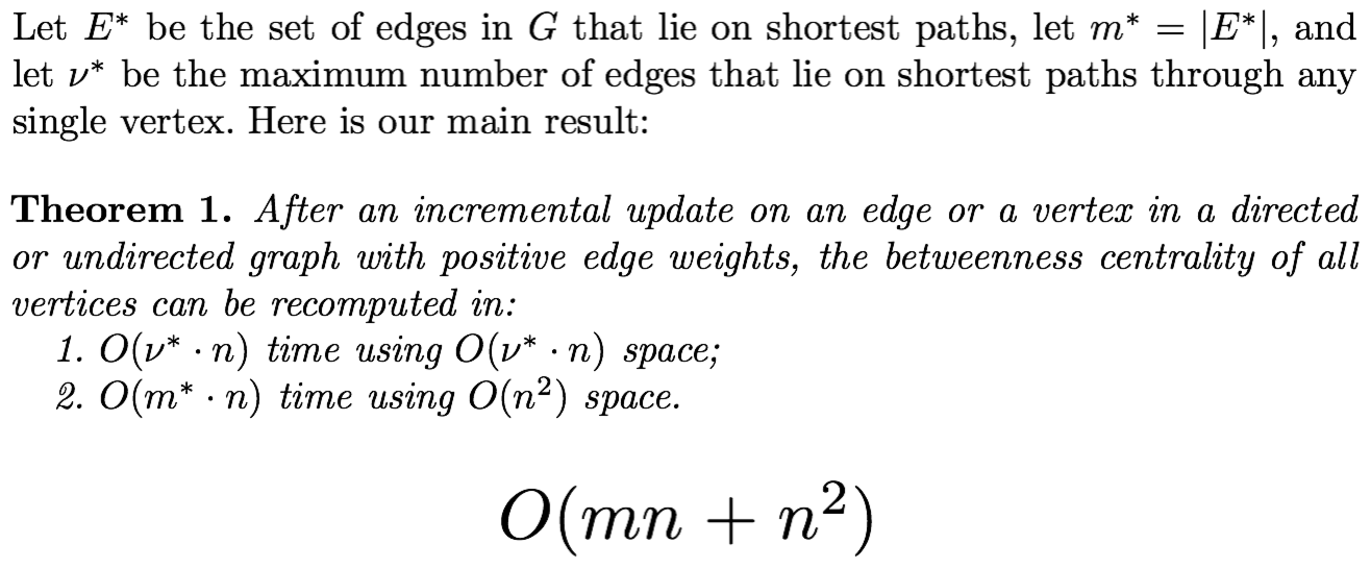
\includegraphics[width=\textwidth]{imgs/npr14-main-result}
  \end{figure}
\end{frame}


\begin{frame}
  \frametitle{Lemmas}

  \begin{figure}[H]
    \centering
    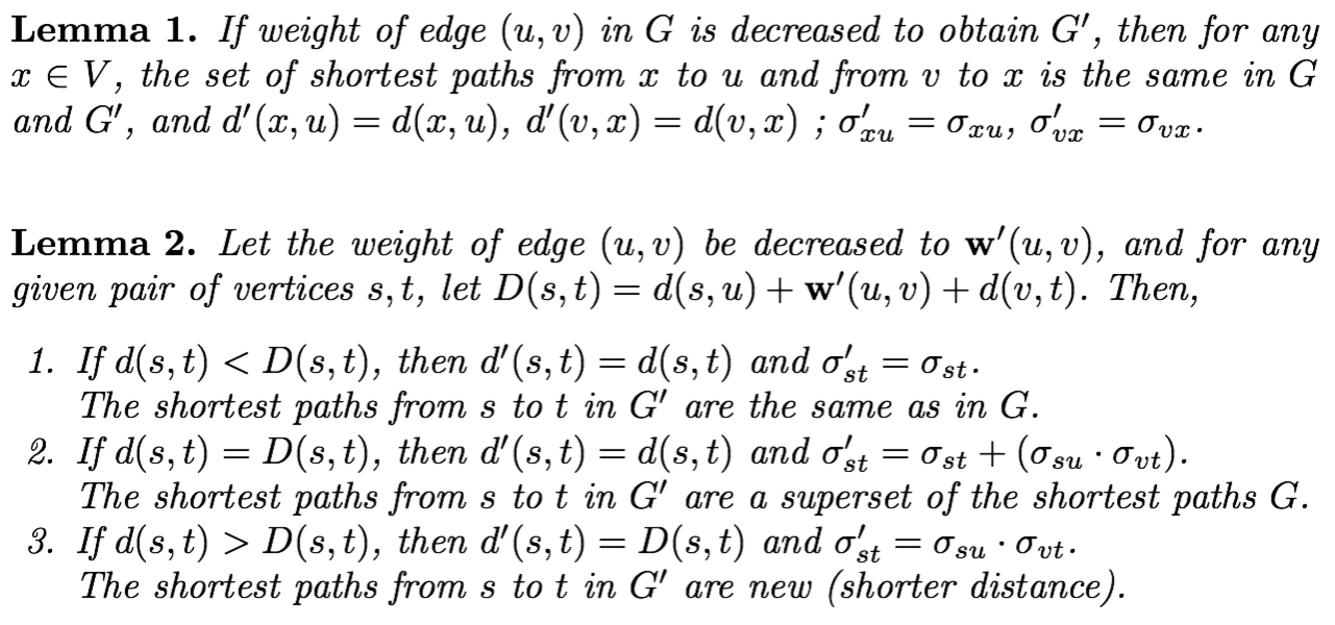
\includegraphics[width=\textwidth]{imgs/npr14-lemmas}
  \end{figure}
\end{frame}


\begin{frame}
  \frametitle{SSSP DAG Update}

  \begin{figure}[H]
    \centering
    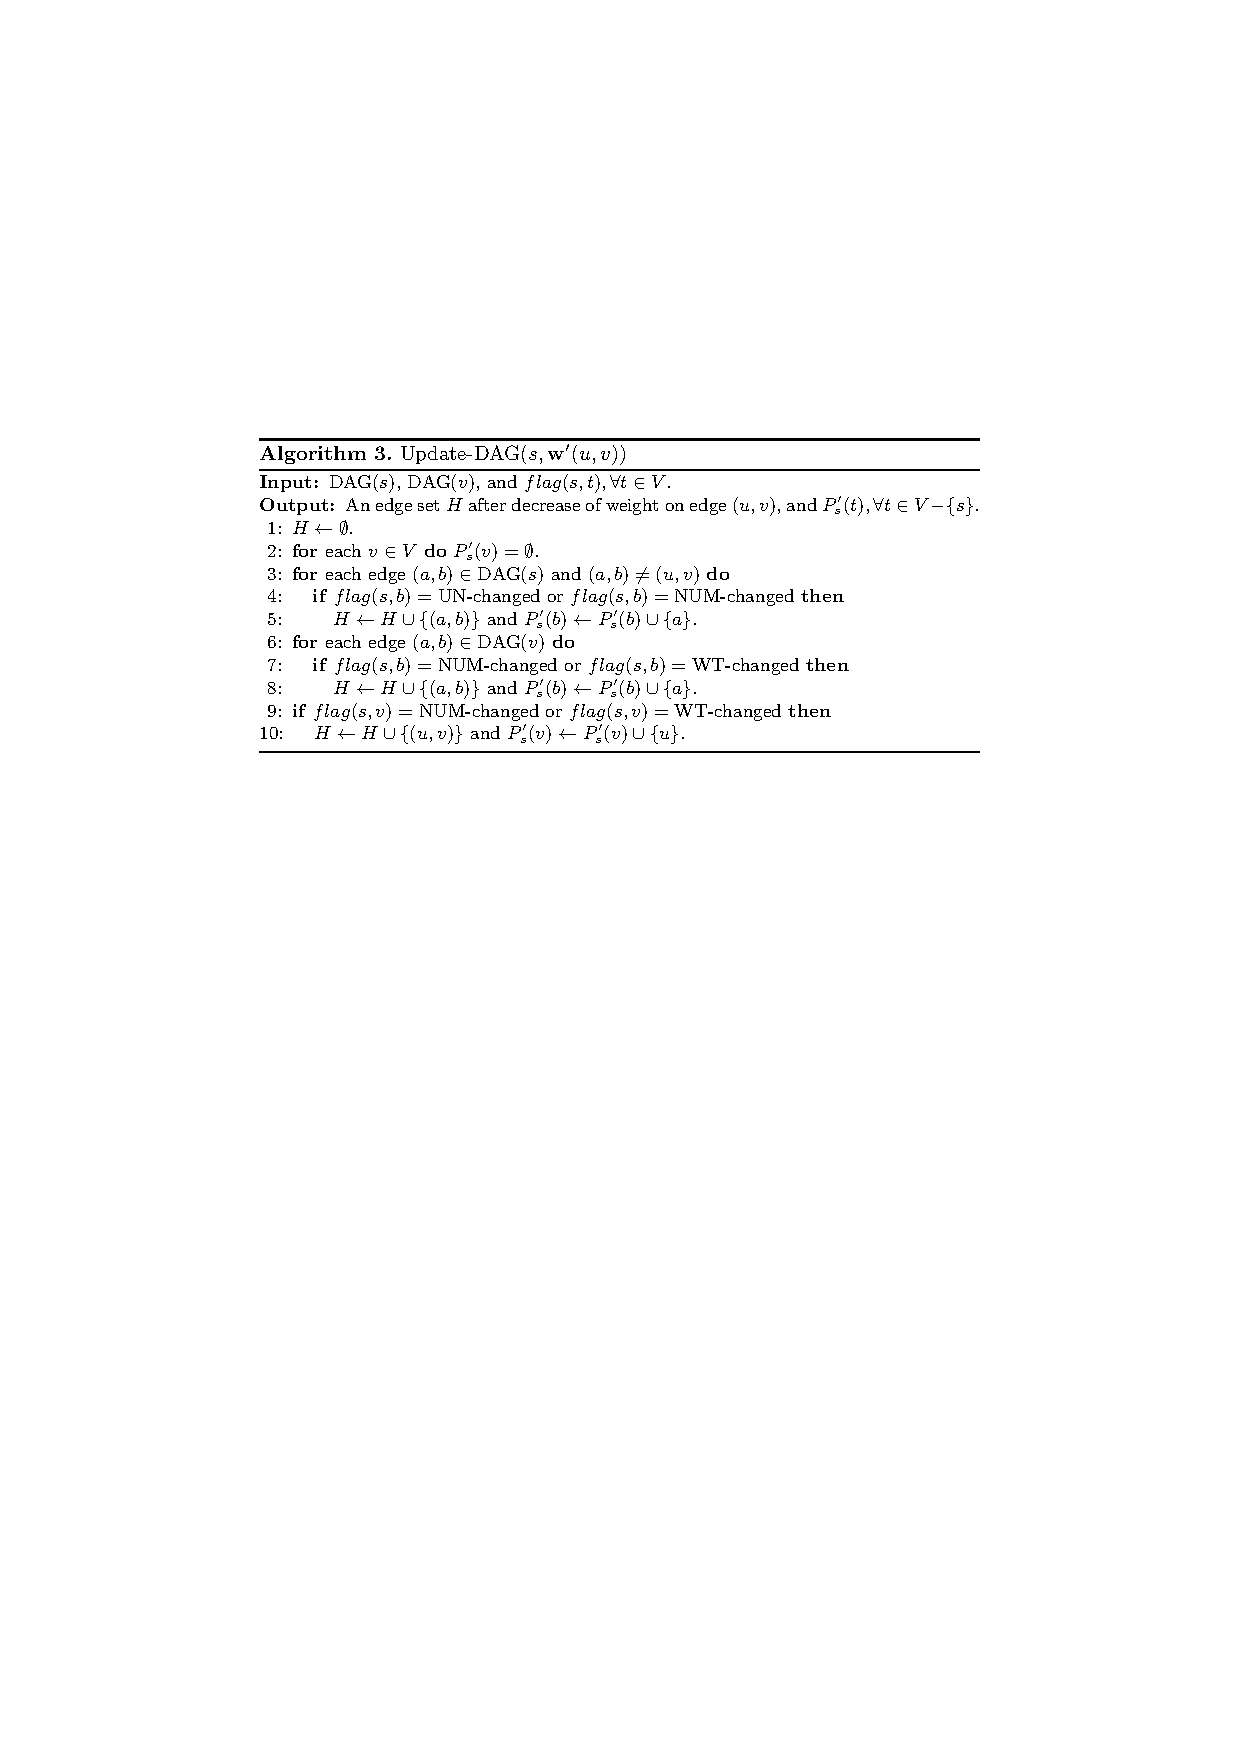
\includegraphics[width=\textwidth]{imgs/npr14-algo3}
  \end{figure}
\end{frame}


\begin{frame}
  \frametitle{Edge Update}

  \begin{figure}[H]
    \centering
    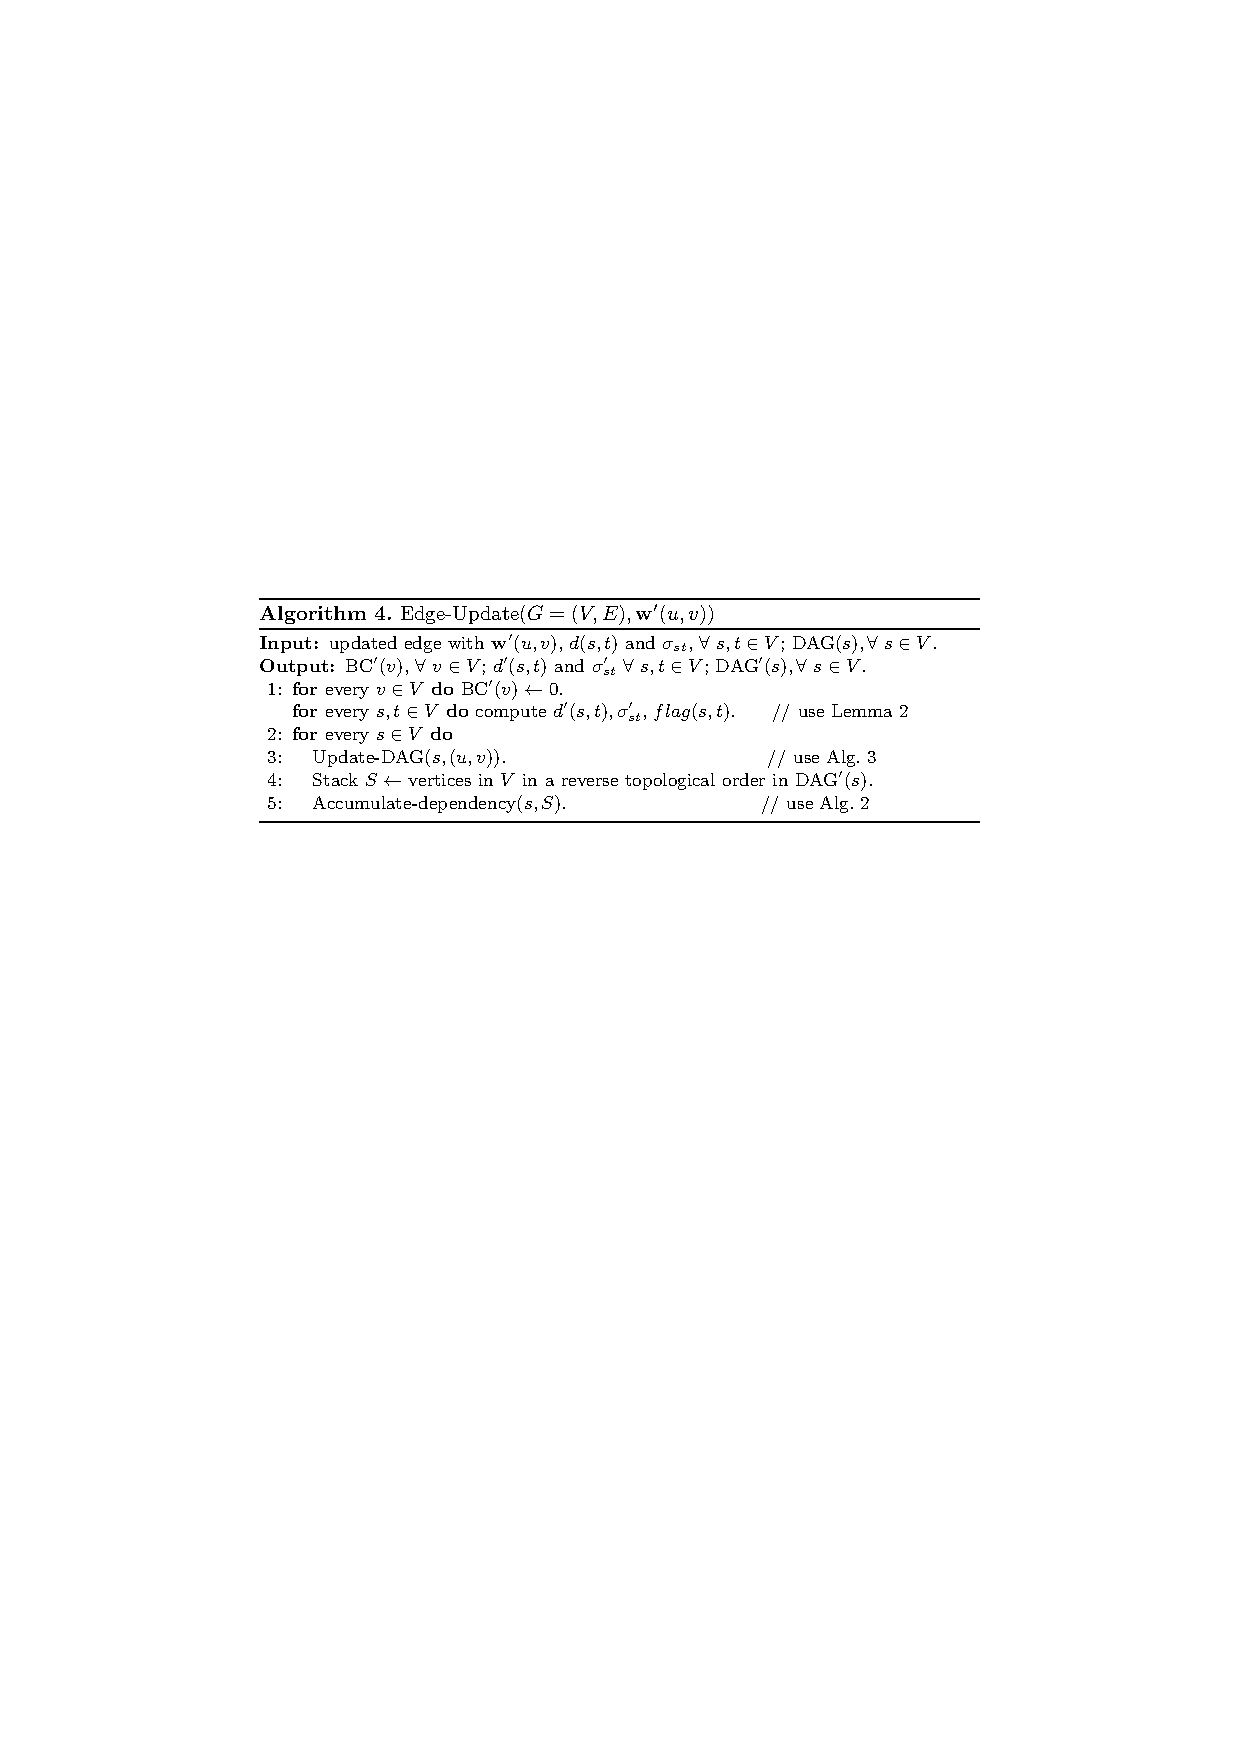
\includegraphics[width=\textwidth]{imgs/npr14-algo4}
  \end{figure}
\end{frame}


\begin{frame}
  \frametitle{Space-Efficient Variant $O(n^2)$}
  
  \begin{itemize}
    \item Do not store the \sssp \dag
    \item Store only $E^*$
    \item Updated \dag can be build in $O(m^*)$ time
    \begin{itemize}
      \item Time $O(m^* \times n)$
      \item Compute ${E'}^*$ from $E^*$, then $\dag'(s)$ from ${E'}^*$
    \end{itemize}
    \item Space $O(m^* + n^2)$ to store $E^*$ and $n^2$ distances $\dist(s,t)$ and shortest paths $\paths_{st}$
  \end{itemize}
\end{frame}


\begin{frame}
  \frametitle{Comparison}

  \begin{figure}[H]
    \centering
    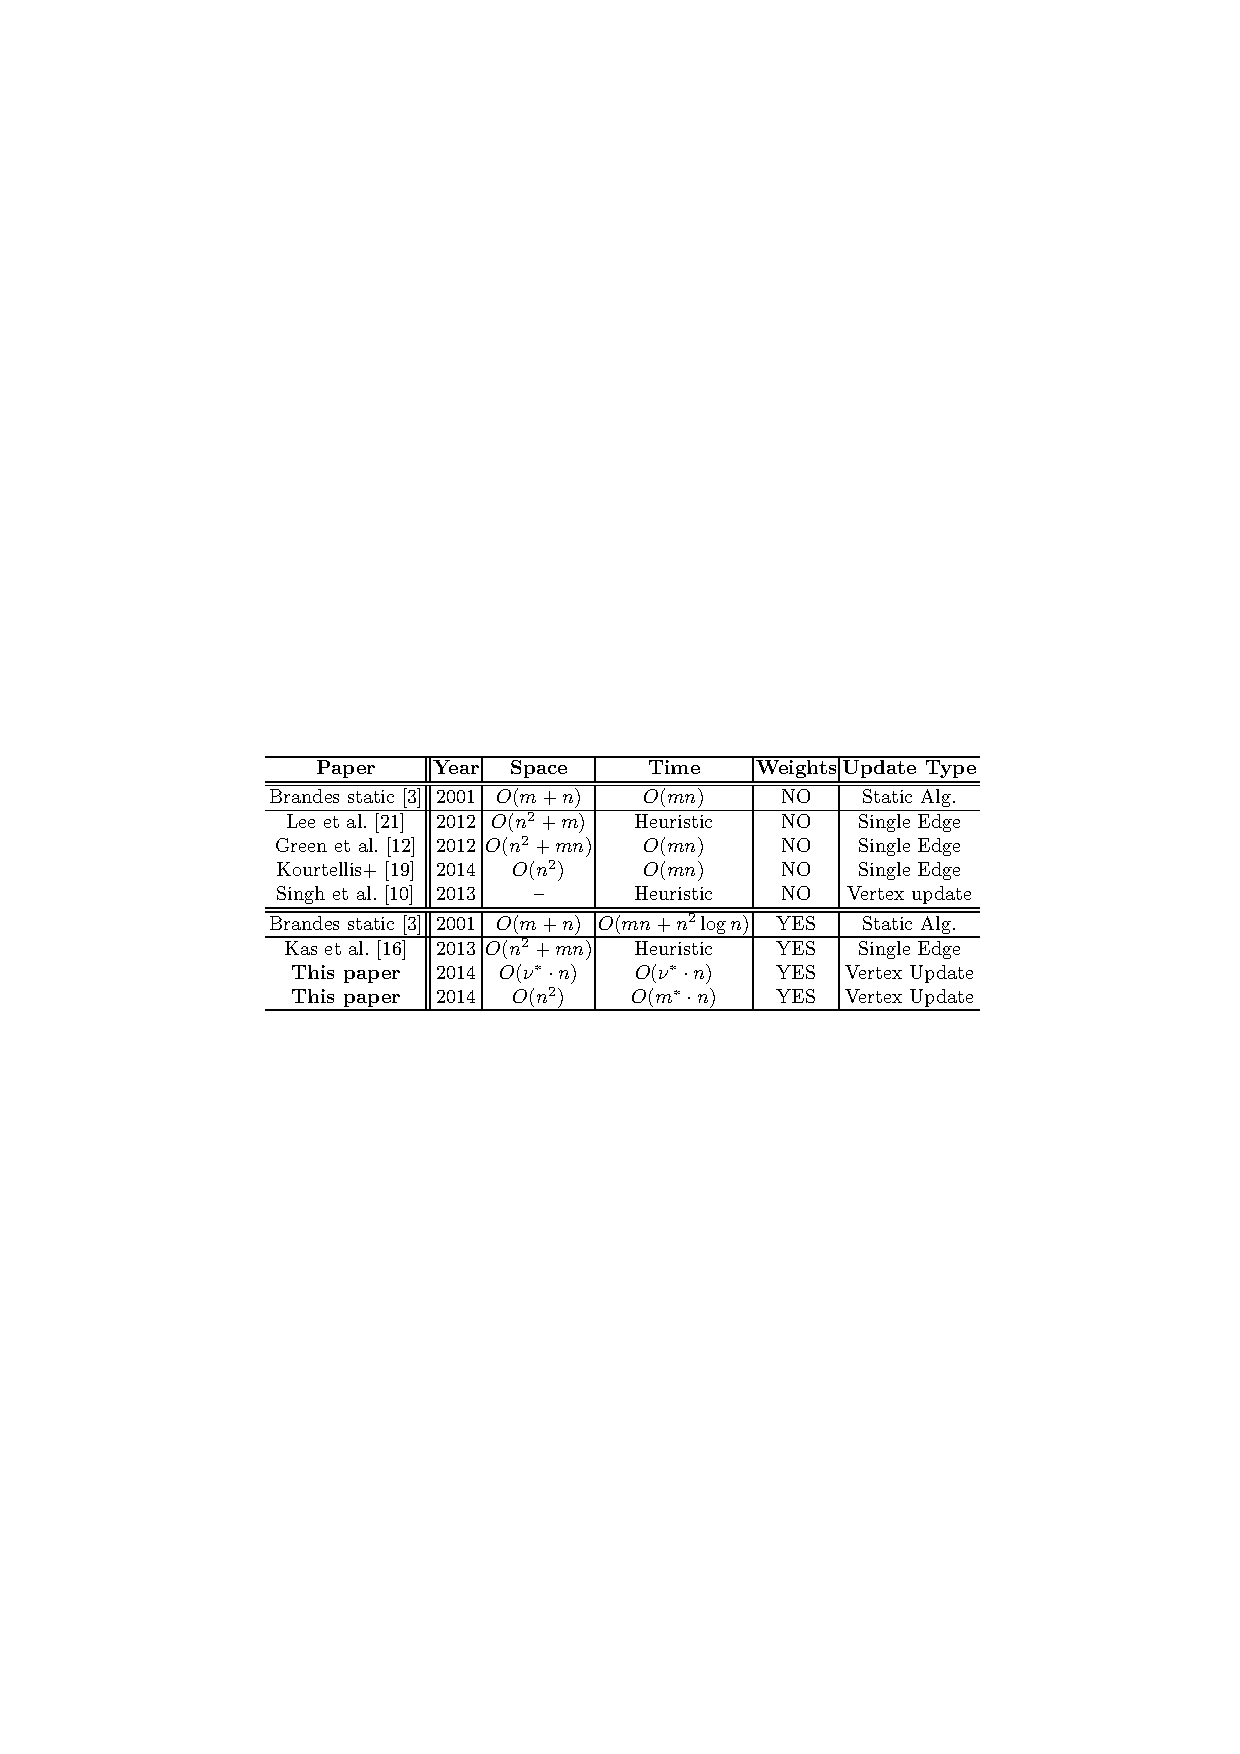
\includegraphics[width=\textwidth]{imgs/npr14-comparison}
  \end{figure}
\end{frame}


\begin{frame}
  \frametitle{Shortcomings}

  \begin{itemize}
    \item Not fully dynamic (no edge removal)
    \item $m^*$ can be large in practice
    \item Non-trivial to parallelize (need to access pairs of \sssp \dag at a time)
    \item Does not solve main bottleneck of most algorithms: $O(n^2)$ memory
  \end{itemize}
\end{frame}


%% Pontecorvi et al.
\begin{frame}
  \frametitle{A Faster Algorithm for Fully Dynamic Betweenness Centrality}
  \centering
  \vfill
  {\huge M. Pontecorvi, V. Ramachandran}
  \vfill
  {\large arXiv:1506.05783}
\end{frame}


%% QUBE
\begin{frame}
  \frametitle{QUBE: a Quick Algorithm for Updating BEtweenness centrality}
  \centering
  \vfill
  {\huge M. Lee, J. Lee, J. Park, R. Choi, C. Chung}
  \vfill
  {\large WWW '12: International World Wide Web Conference}
\end{frame}

\begin{frame}
  \frametitle{Intuition}
  
  \begin{itemize}
    \item No need to update all vertices when a new edge is added
    \item Prune vertices whose \betw does not change
    \item Large reduction in all-pairs shortest paths to be re-computed
  \end{itemize}
\end{frame}


\begin{frame}
  \frametitle{Minimum Cycle Basis}
  
  \begin{itemize}
    \item $G=(V,E)$ undirected graph
    \item \emph{Cycle} $C \subseteq E$ s.t. $\forall v \in V$, $v$ incident to even number of edges in $C$
    \item Represented as edge incidence vector $\nu \in \{ 0,1 \}^{|E|}$, where $\nu(e) = 1 \iff e \in C$ 
    \item \emph{Cycle Basis} = set of linearly independent cycles
    \item \emph{Minimum Cycle Basis} = on weighted graph with non-negative weights $w_e$, cycle basis of minimum total weight $w(C) = \sum_{i} w(C_i)$ where $w(C_i) = \sum_{e \in C_v} w_e$
  \end{itemize}  
\end{frame}


\begin{frame}
  \frametitle{Minimum Cycle Basis Example}
  \begin{itemize}
    \item Three cycle basis sets: $\{C_1, C_2\} , \{C_1, C_3\} , \{C_2, C_3\}$
    \item If all edges have same weight $w_e = 1$, $MCB = \{C_1, C_2\}$
  \end{itemize}
  \begin{figure}[H]
    \centering
    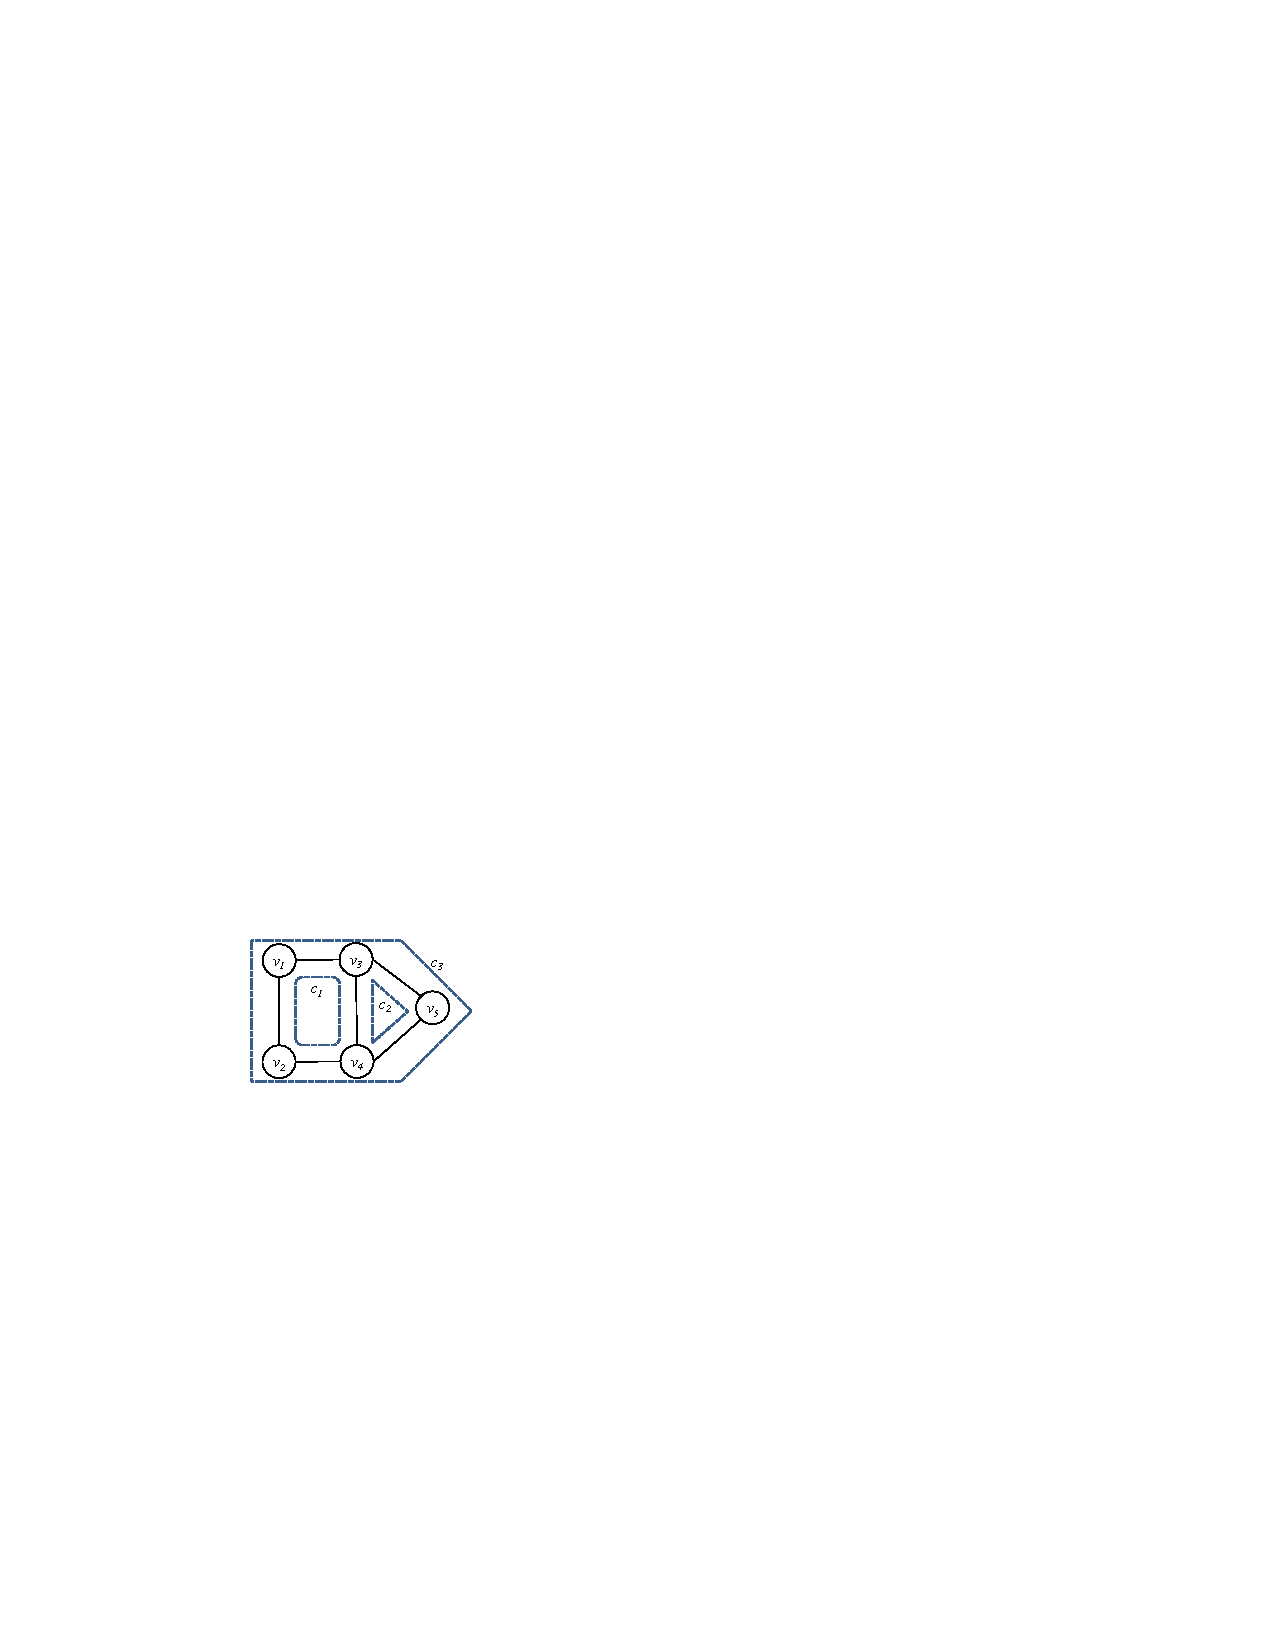
\includegraphics[scale=2]{imgs/qube-mcb}
  \end{figure}
\end{frame}


\begin{frame}
  \frametitle{Minimum Union Cycle}
  
  \begin{itemize}
    \item Given a MCB $C$ and minimum cycles $C_i \in C$
    \item Let $V_{C_i}$ be the set of vertices induced by $C_i$
    \item Recursively union two $V_{C_i}$ if they share at least one vertex
    \item The final set of vertices is a \emph{Minimum Union Cycle} $MUC$
  \end{itemize}
  
  \begin{itemize}
    \item $MUC$s are disjoint sets of vertices
    \item $MUC(v)$ = the $MUC$ which contains vertex $v$
  \end{itemize}
\end{frame}


\begin{frame}
  \frametitle{Connection Vertex}
  
  \begin{itemize}
    \item \emph{Articulation Vertex} = vertex $v$ whose deletion makes the graph disconnected
    \item Biconnected graph = graph with no articulation vertex
    \item Vertex $v$ is an articulation vertex $\iff$ v belongs to two biconnected components
  \end{itemize} 
  
  \begin{itemize}
    \item \emph{Connection Vertex} = vertex $v$ that
    \begin{itemize}
      \item is an articulation vertex
      \item has an edge to vertex $w \not\in MUC(v)$
    \end{itemize} 
  \end{itemize}
\end{frame}


\begin{frame}
  \frametitle{Connection Vertex Example}
  
  \begin{columns}[onlytextwidth]
    \begin{column}{0.5\textwidth}
      \begin{itemize}
        \item If $(v_3, v_4)$ is added, $MUC(v_3) = \{ v_1, v_2, v_3, v_4 \}$
        \item $v_1, v_2, v_3$ are connection vertices of $MUC(v_3)$
        \item Let $G_i$ be the disconnected subgraph generated by removing $v_i$
      \end{itemize}
    \end{column}
    
    \begin{column}{0.5\textwidth}
      \begin{figure}[t]
        \centering
        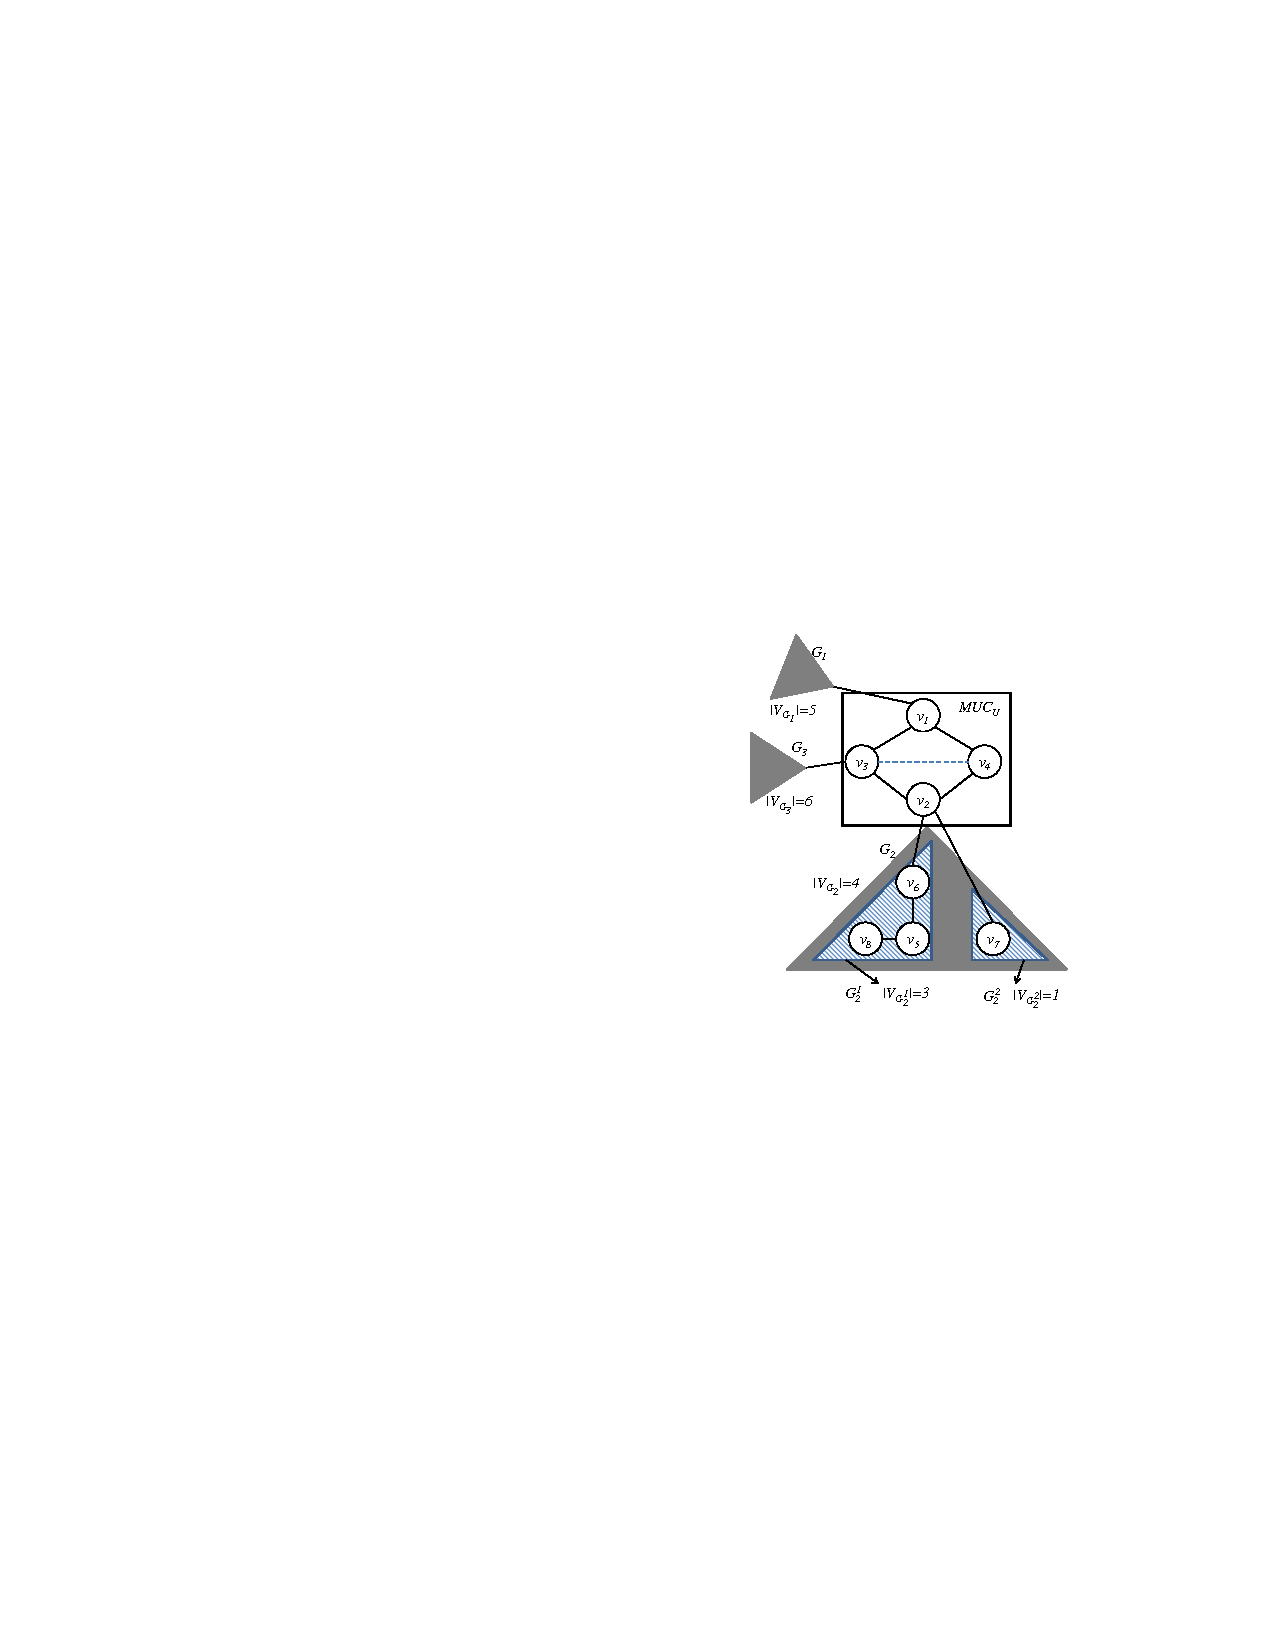
\includegraphics[width=\textwidth, height=0.8\textheight, keepaspectratio]{imgs/qube-biconnected}
      \end{figure}
    \end{column}
  \end{columns}
  
\end{frame}


\begin{frame}
  \frametitle{Finding MUCs}
  
  \begin{itemize}
    \item Finding an $MCB$ is well studied
    \item Kavitha, Mehlhorn, Michail, Paluch. ``A faster algorithm for minimum cycle basis of graphs''. ICALP 2004
    \item Finding $MUC$ from $MCB$ relatively straightforward (just union sets of vertices)
    \item Also find connection vertices for each $MUC$
    \item All done as a preprocessing step
    \item Need to be updated at runtime
  \end{itemize}
\end{frame}


\begin{frame}
  \frametitle{Updating MUCs -- Addition}
  
  \begin{figure}[t]
    \centering
    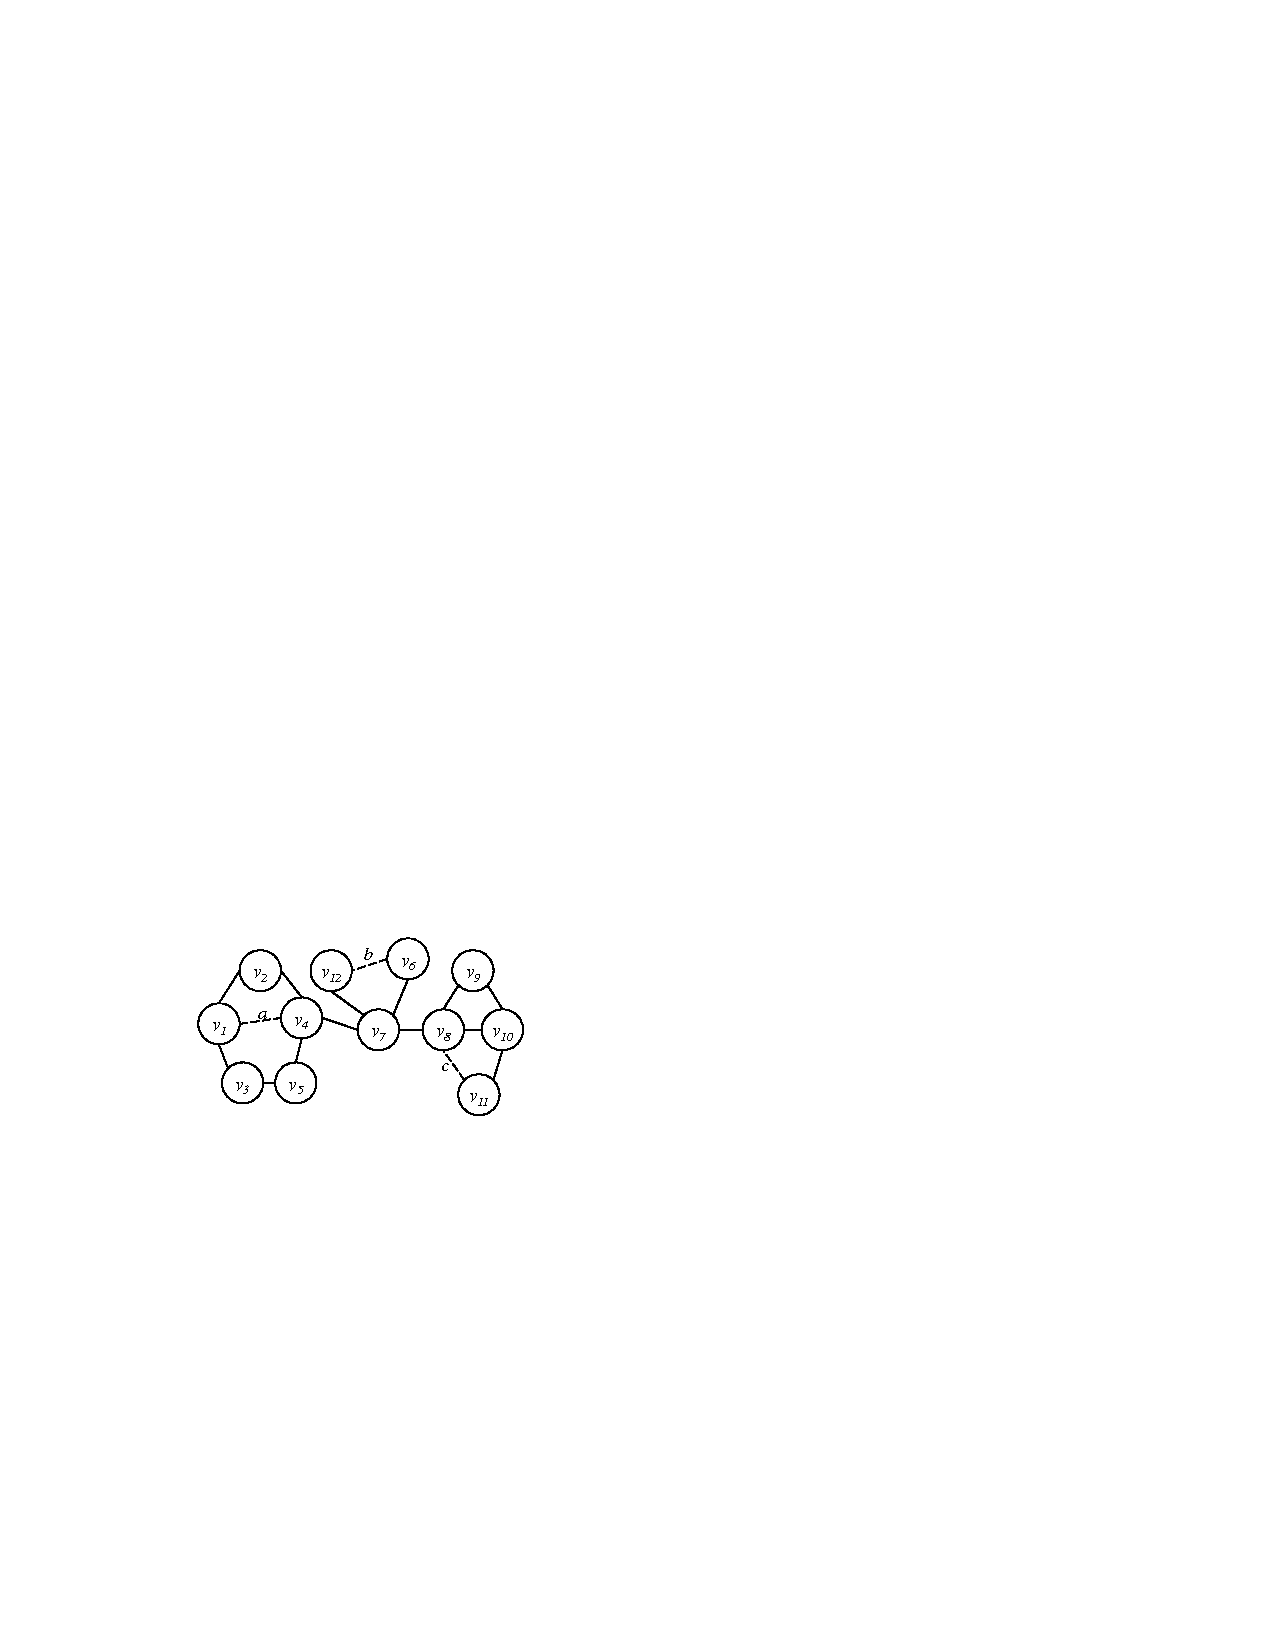
\includegraphics[width=\textwidth, height=0.6\textheight, keepaspectratio]{imgs/qube-addition}
  \end{figure}
    
  \begin{itemize}
    \item Adding $a$ does not affect the $MUC$ (endpoints in the same $MUC$)
    \item Adding $b$ creates a new $MUC$ (endpoints do not belong to a $MUC$)
    \item Adding $c$ merges two $MUC$s (merge $MUC$s of vertices on the \spath between endpoints)
  \end{itemize}
\end{frame}


\begin{frame}
  \frametitle{Updating MUCs -- Removal}
  
  \begin{figure}[t]
    \centering
    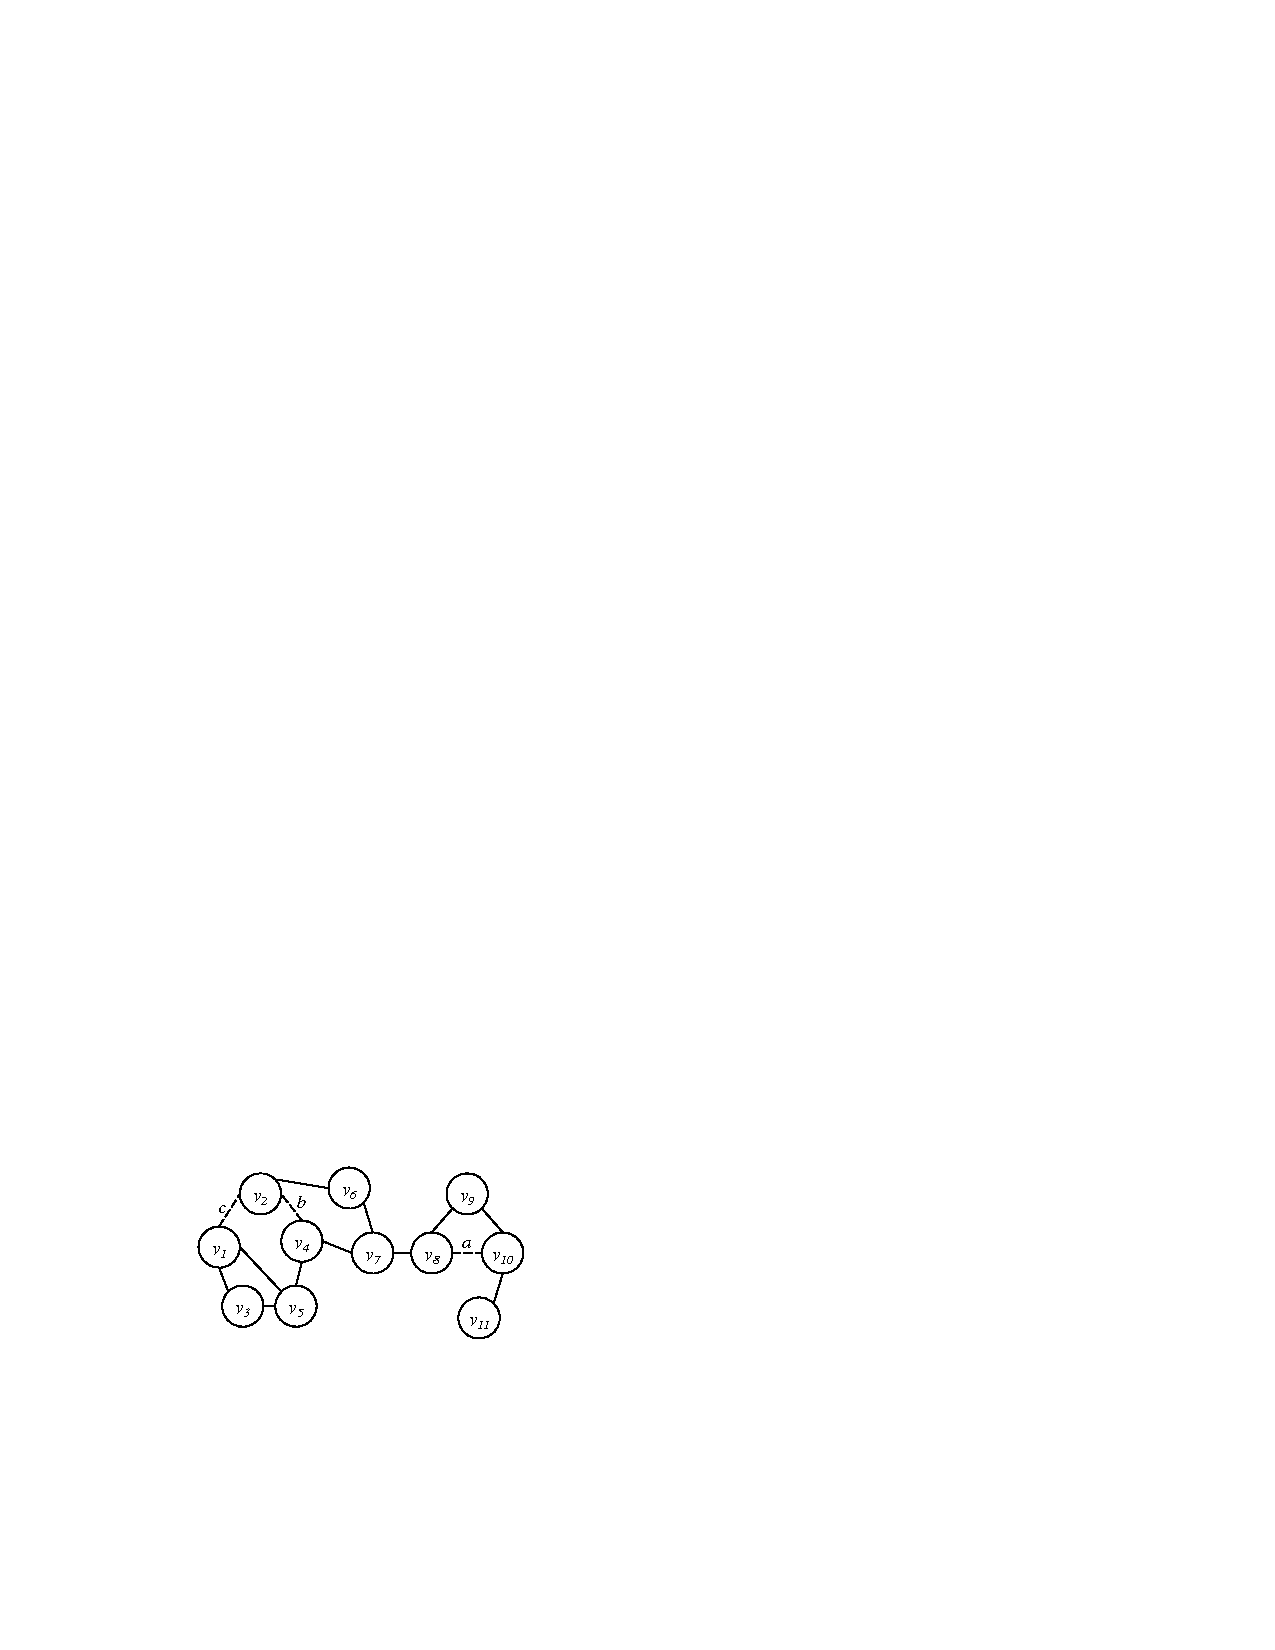
\includegraphics[width=\textwidth, height=0.6\textheight, keepaspectratio]{imgs/qube-removal}
  \end{figure}
  
  \begin{itemize}
    \item Removing $a$ destroys the $MUC$ (cycle is removed $\rightarrow$ no biconnected component)
    \item Removing $b$ does not affect the $MUC$ ($MUC$ is still biconnected)
    \item Removing $c$ splits the $MUC$ in two (single vertex appears in all \spath between endpoints)
  \end{itemize}    
\end{frame}


\begin{frame}
  \frametitle{Betweenness Centrality Dependency}
  
  \begin{itemize}
    \item Only vertexes inside the $MUC$s of the updated endpoints need to be updated
    \item However, recomputing all centralities for the $MUC$ still requires new shortest paths to the rest of the graph
      \begin{itemize}
        \item Shortest paths to vertices outside the $MUC$
        \item Shortest paths that pass through the $MUC$
      \end{itemize}
  \end{itemize}
  
  \begin{figure}[t]
    \centering
    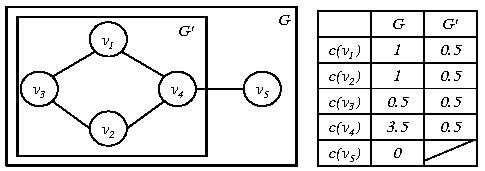
\includegraphics[width=\textwidth, height=0.6\textheight, keepaspectratio]{imgs/qube-btwmuc}
  \end{figure}
\end{frame}


\begin{frame}
  \frametitle{Betweenness Centrality outside the MUC}
  
  \begin{itemize}
    \item Let $s \in V_{G_j}$, $t \in MUC$,
    \item Let $j \in MUC$ be a connection vertex to subgraph $G_j$
    \item Each vertex in $\spath_{jt}$ is also in $\spath_{st}$
    \item Therefore, betweenness centrality due to vertices outside the $MUC$:    
  \end{itemize}
  
  \begin{align*}
    \large
    \betw_{o}(v) = \begin{cases}
      \frac{|V_{G_j}|}{\paths_{st}}		& \text{ if } v \in\{ \spath_{ct} \setminus t \} \\
      0 						& \text{ otherwise }
    \end{cases}
  \end{align*}
\end{frame}


\begin{frame}
  \frametitle{Betweenness Centrality trough the MUC}
  
  \begin{itemize}
    \item Let $s \in V_{G_j}$, $t \in V_{G_k}$,
    \item Let $j \in MUC$ be a connection vertex to subgraph $G_j$
    \item Let $k \in MUC$ be a connection vertex to subgraph $G_k$
    \item Each vertex in $\spath_{jk}$ is also in $\spath_{st}$
    \item Therefore, betweenness centrality due to paths through the $MUC$:    
  \end{itemize}

  \begin{align*}
    \betw_{x}(v) = \begin{cases}
      \frac{ |V_{G_j}| |V_{G_k}| }{ \paths_{st} }		& \text{ if } v \in \spath_{jk} \\
      0 						& \text{ otherwise }
    \end{cases}
  \end{align*}
  
  More caveats apply for subgraphs that are disconnected, as every path that connects vertices in different connected component passes through $v$
\end{frame}


\begin{frame}
  \frametitle{Updating Betweenness Centrality}
  
  {\huge
  \begin{align*}
    \betw(v) = \betw_{MUC}(v) + \sum_{G_j \subset G} \betw_{o}(v) + \sum_{G_j, G_k \subset G} \betw_{x}(v)
  \end{align*}
  }
\end{frame}


\begin{frame}
  \frametitle{Updating MUCs -- Removal}
  
  \begin{figure}[t]
    \centering
    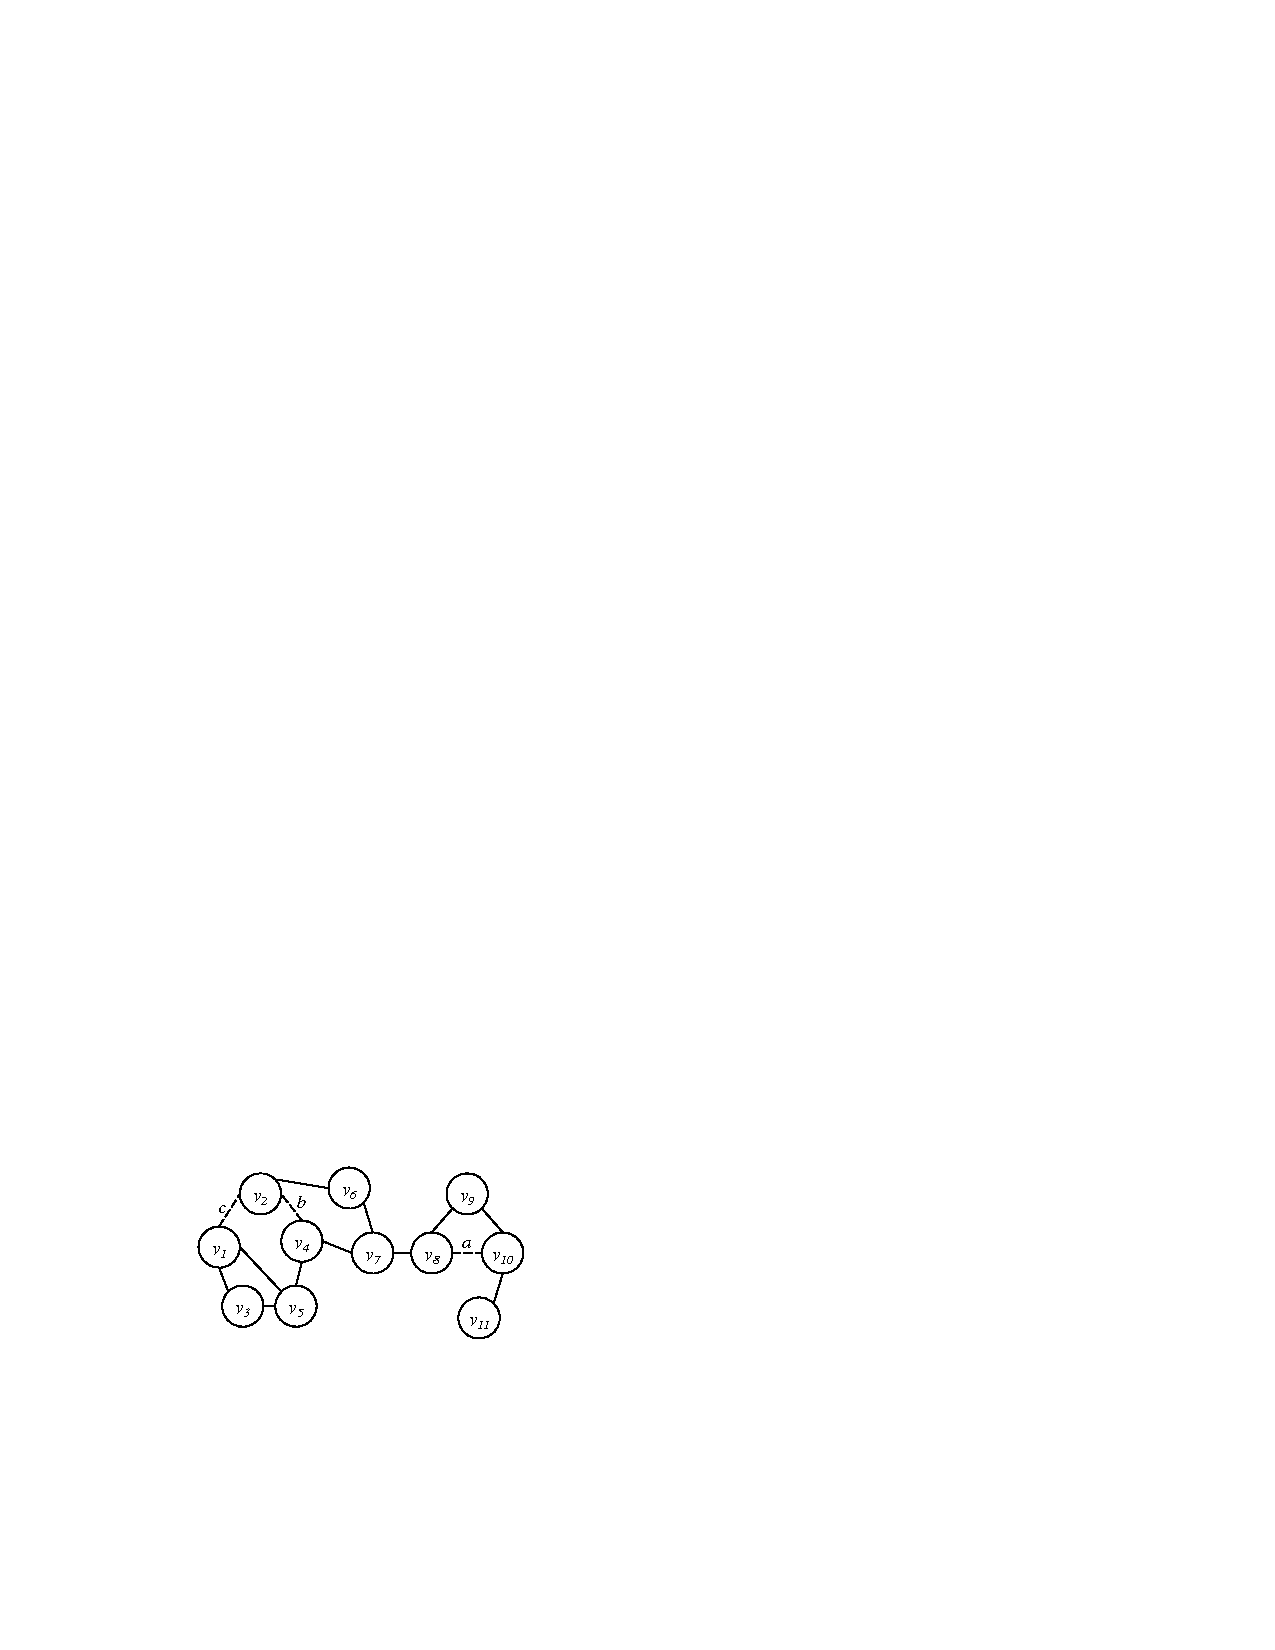
\includegraphics[width=\textwidth, height=0.6\textheight, keepaspectratio]{imgs/qube-removal}
  \end{figure}
\end{frame}
  

\begin{frame}
  \frametitle{QUBE algorithm}

      \begin{figure}[t]
        \centering
        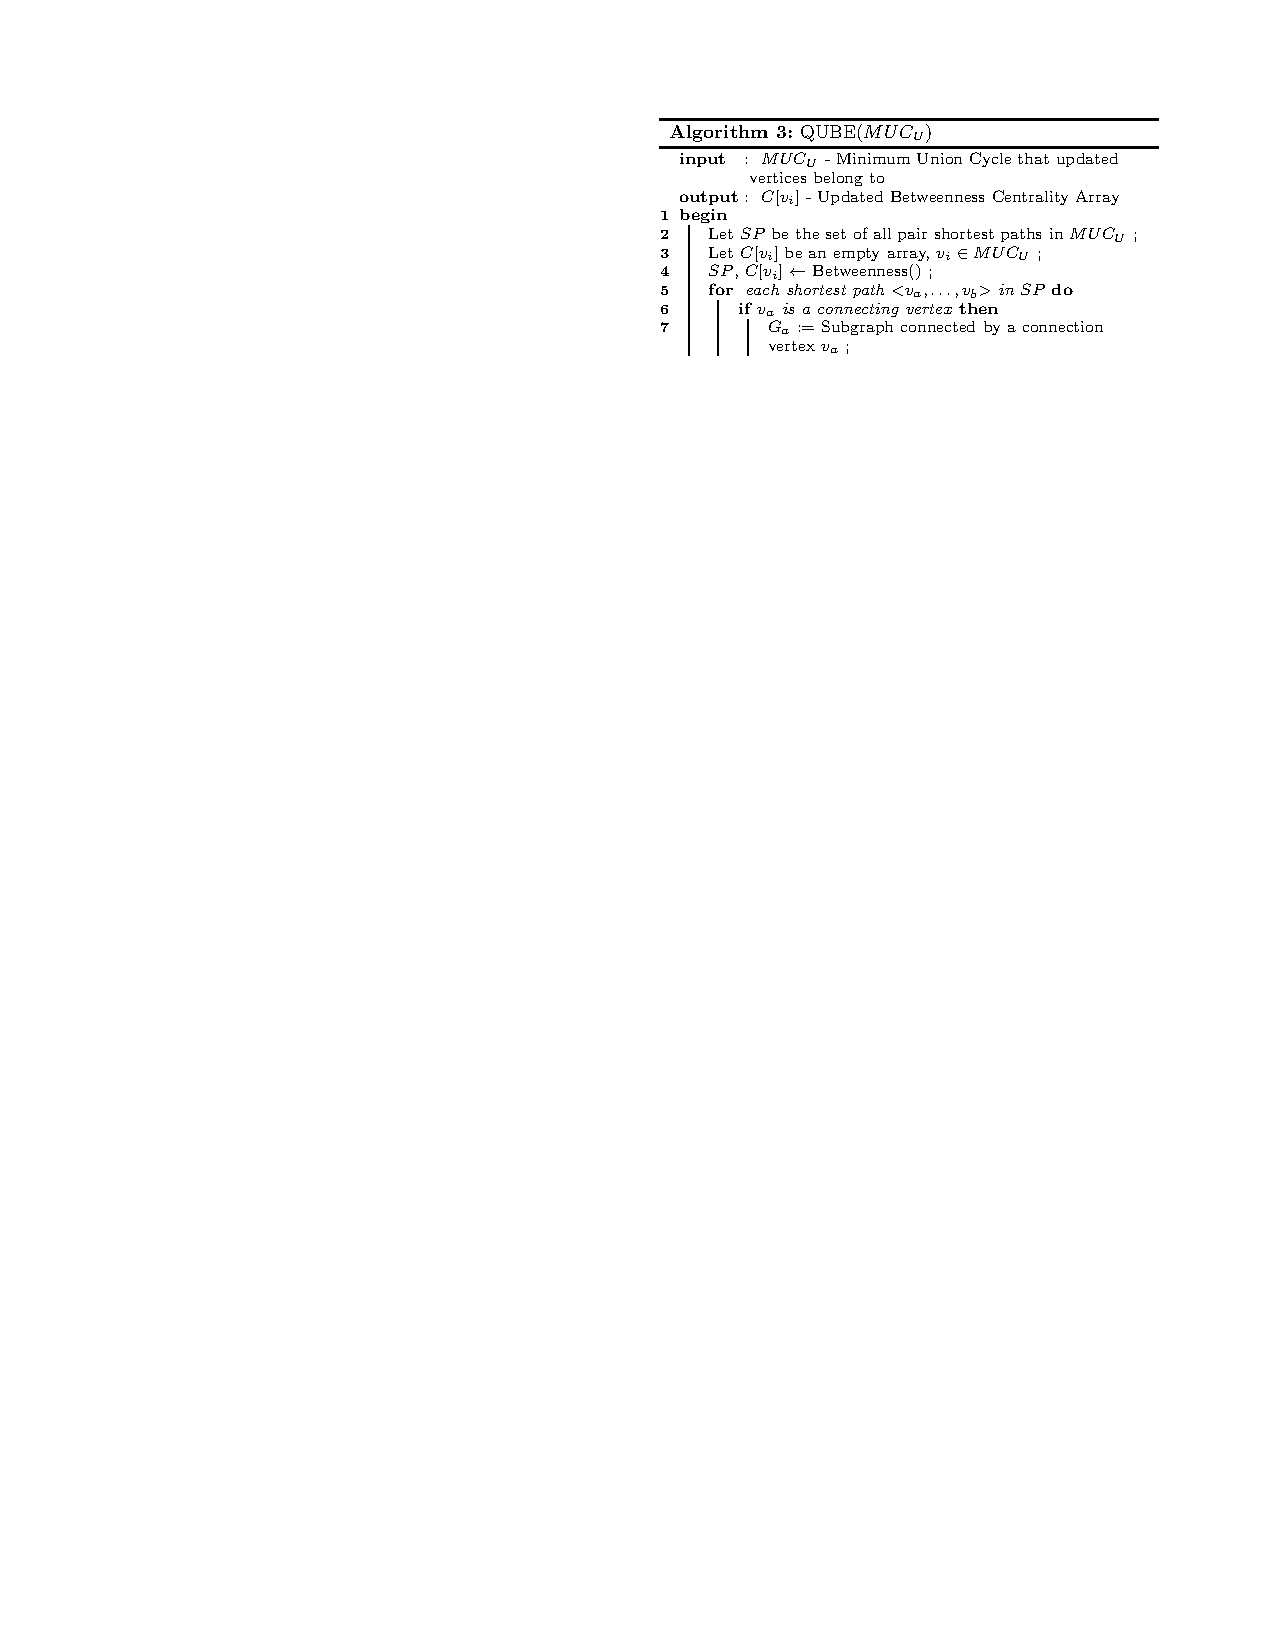
\includegraphics[width=\textwidth, height=\textheight, keepaspectratio]{imgs/qube-algorithm1}
      \end{figure}

%  \begin{columns}[onlytextwidth]
%    \begin{column}{0.5\textwidth}
%      \begin{figure}[t]
%        \centering
%        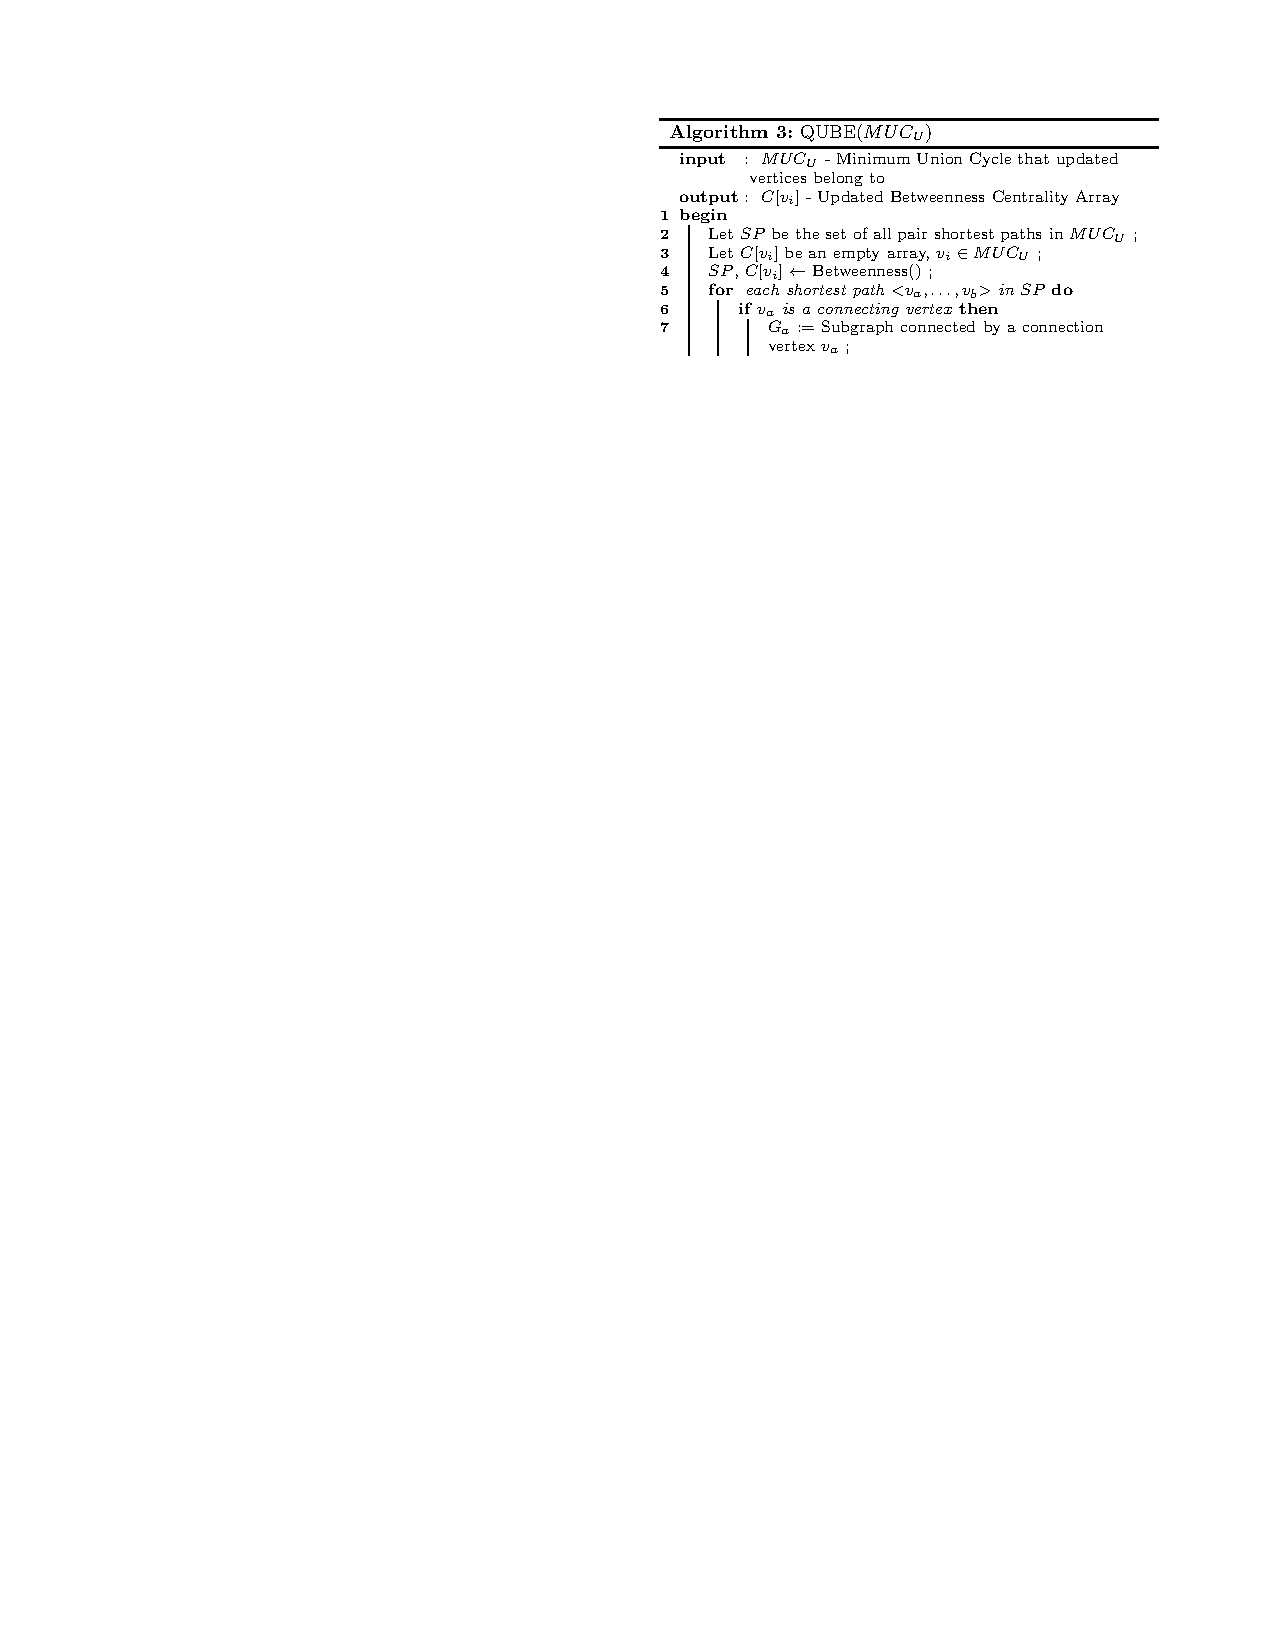
\includegraphics[width=\textwidth, height=\textheight, keepaspectratio]{imgs/qube-algorithm1}
%      \end{figure}
%    \end{column}
    
%    \begin{column}{0.5\textwidth}
%      \begin{figure}[t]
%        \centering
%        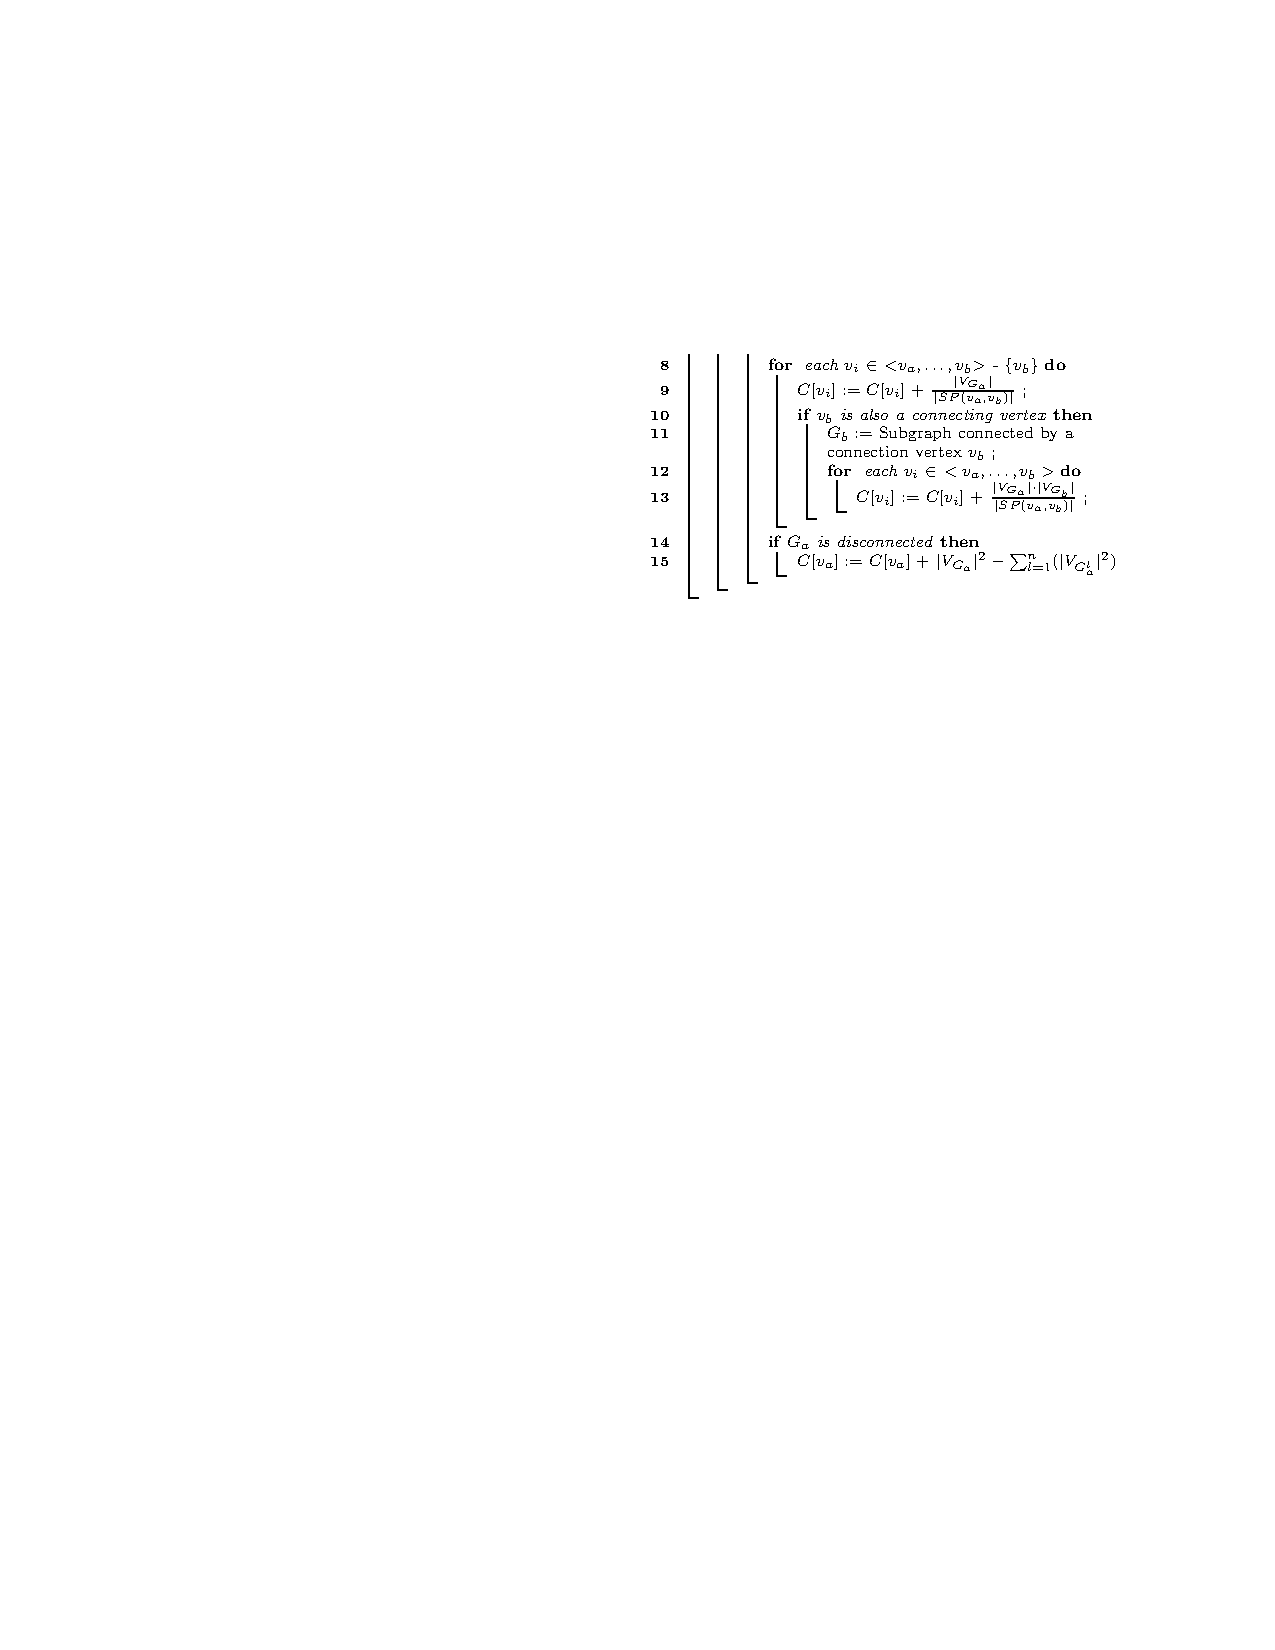
\includegraphics[width=\textwidth, height=\textheight, keepaspectratio]{imgs/qube-algorithm2}
%      \end{figure}
%    \end{column}
%  \end{columns}
\end{frame}


\begin{frame}
  \frametitle{QUBE algorithm}

      \begin{figure}[t]
        \centering
        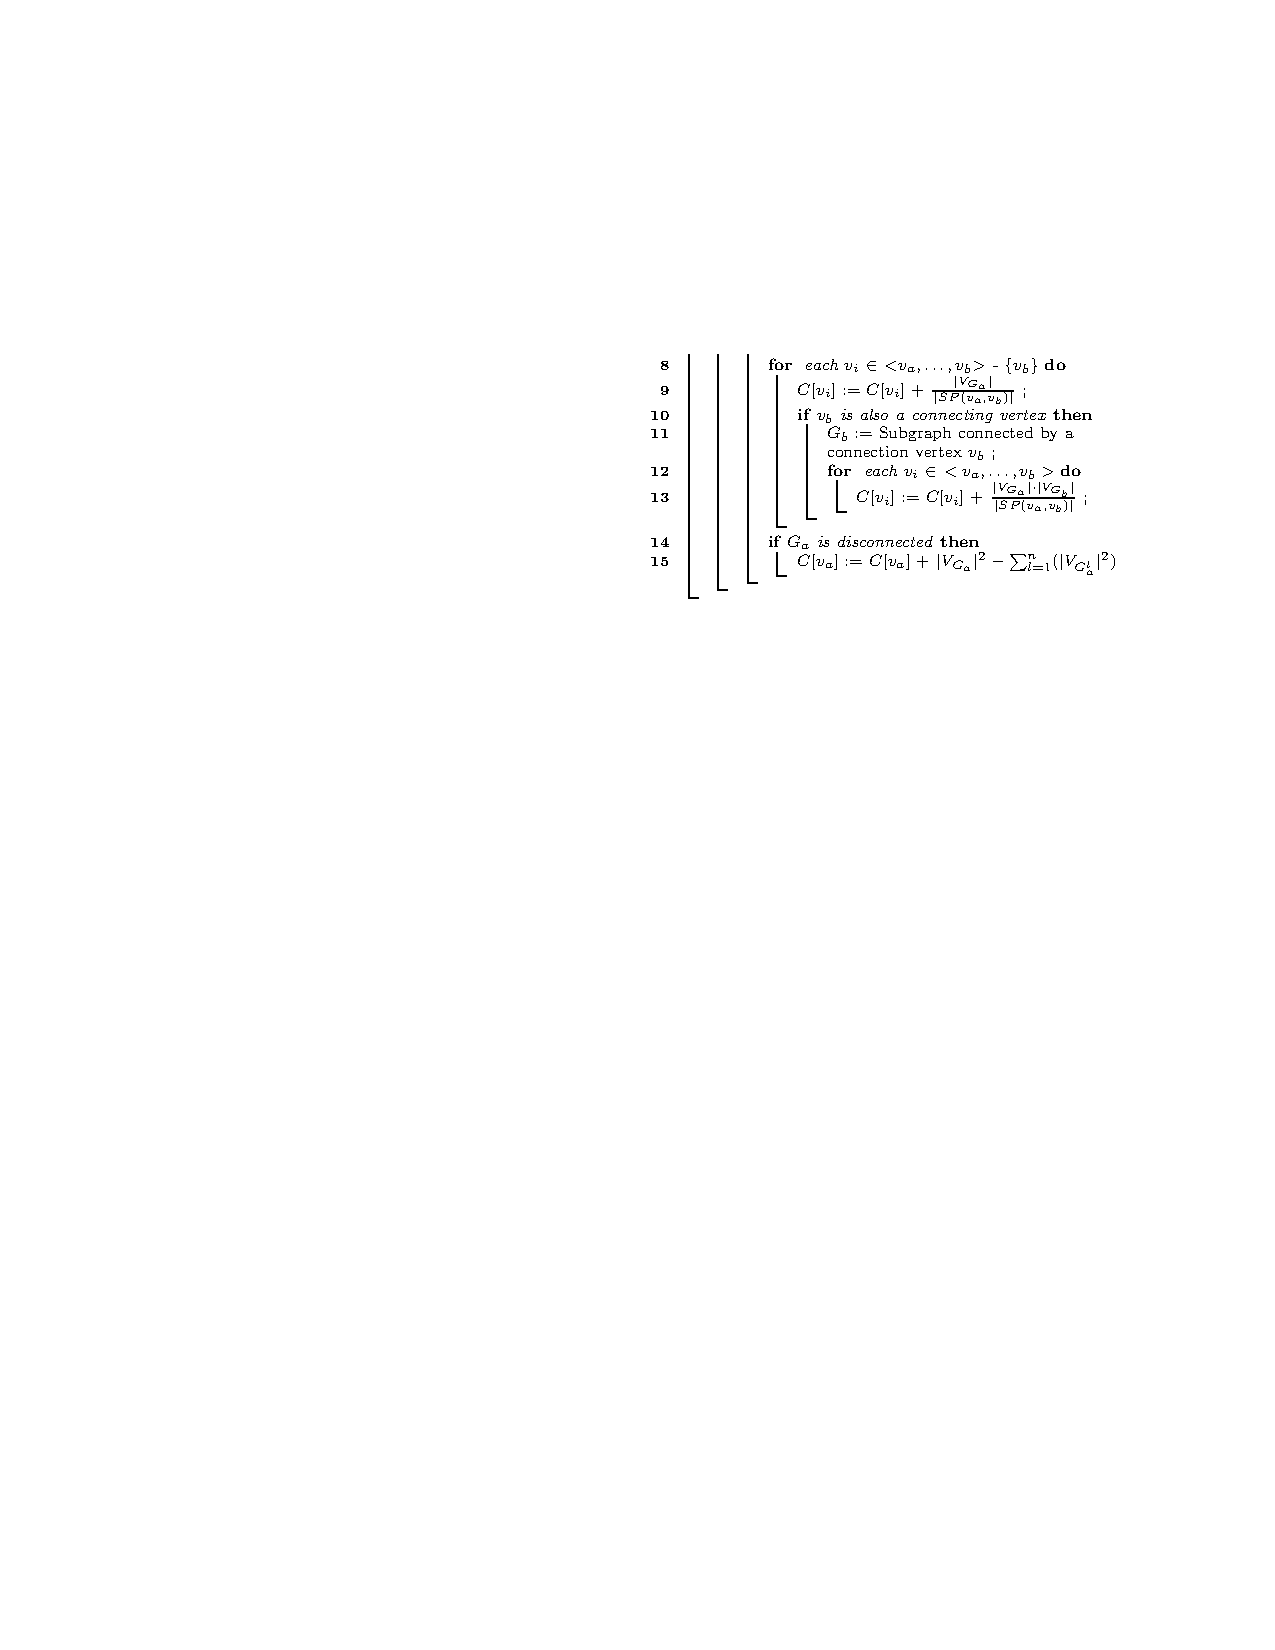
\includegraphics[width=\textwidth, height=\textheight, keepaspectratio]{imgs/qube-algorithm2}
      \end{figure}
      
\end{frame}


\begin{frame}
  \frametitle{QUBE + Brandes}
  
  \begin{itemize}
    \item QUBE is a pruning rule that reduces the search space for betweenness recomputation
    \item Can be paired with any existing betweenness algorithm to compute $\betw_{MUC}$
    \item In the experiments, Brandes' is used
    \item Quantities computed by Brandes' (e.g., \paths) reused by QUBE for $\betw_o$ and $\betw_x$
  \end{itemize}
\end{frame}


\begin{frame}
  \frametitle{Results}

  \begin{figure}[t]
    \centering
    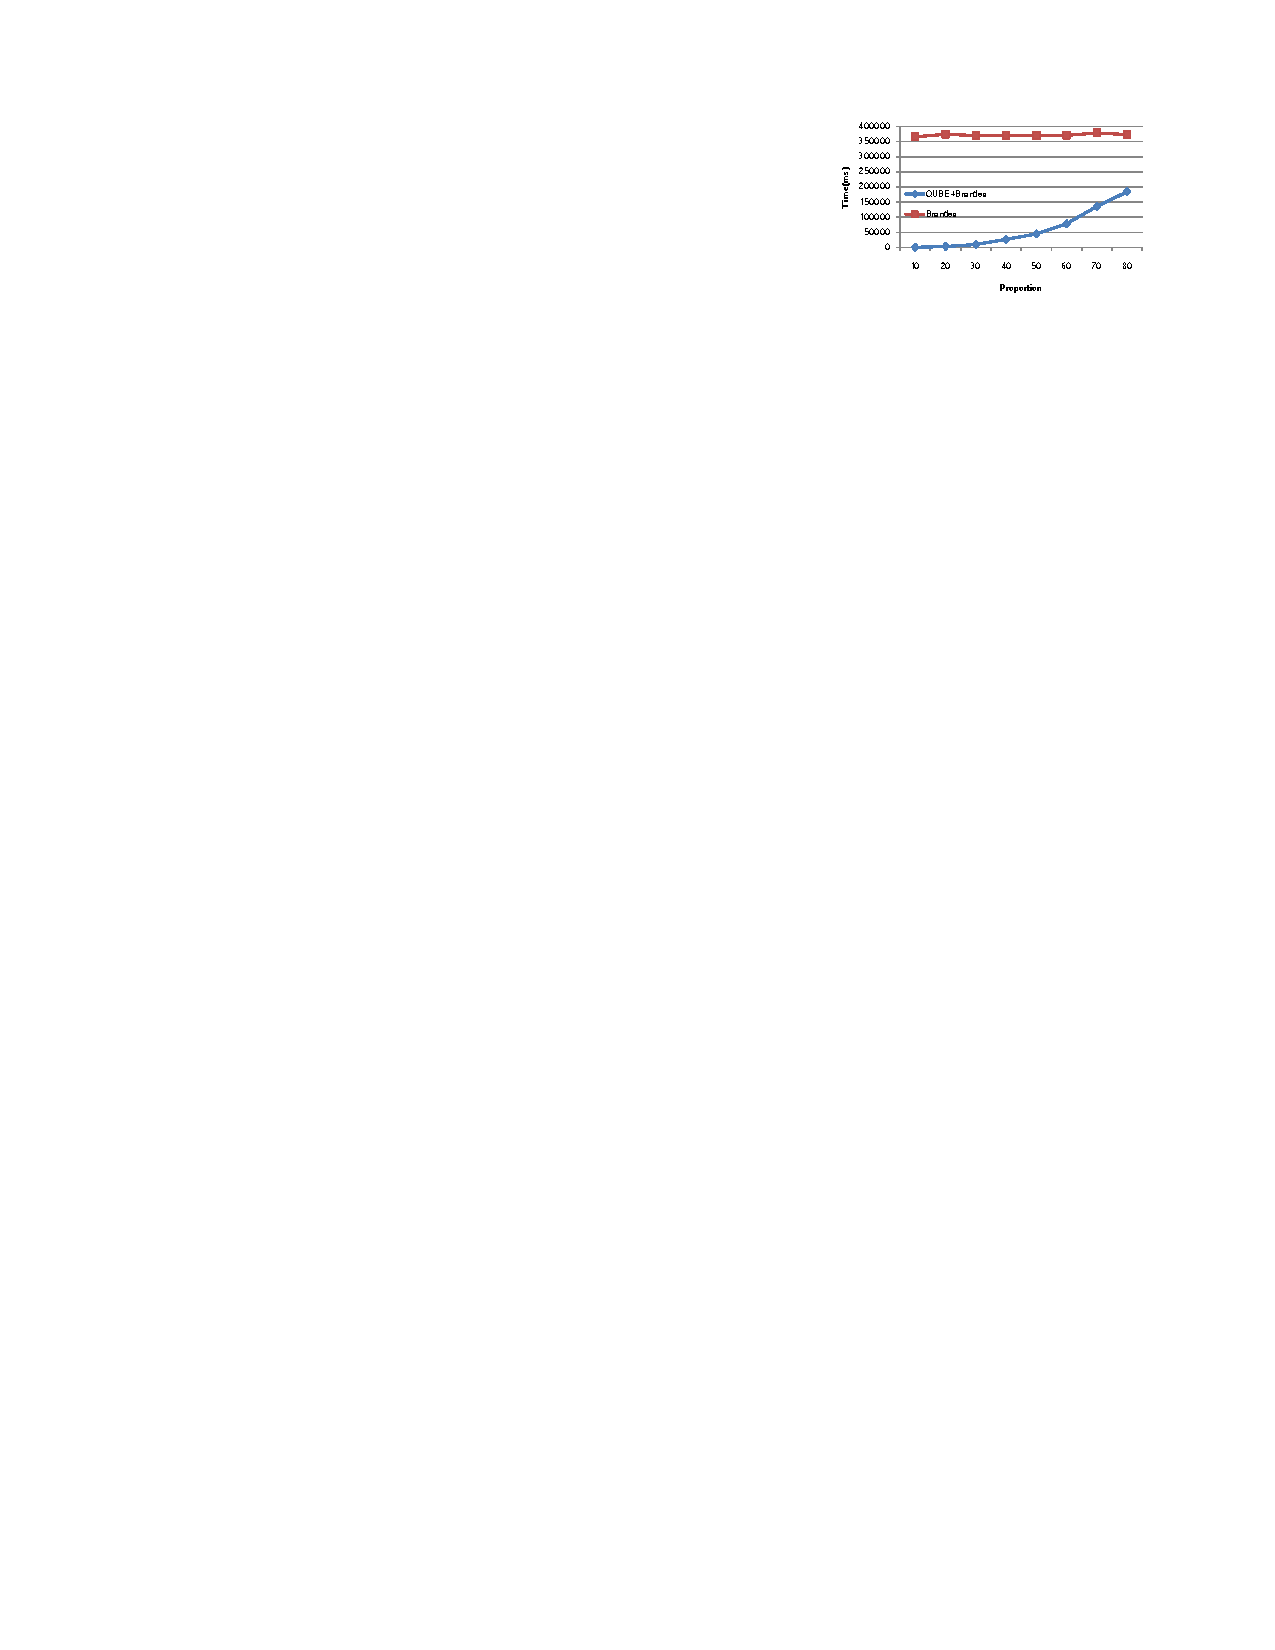
\includegraphics[width=\textwidth, height=0.7\textheight, keepaspectratio]{imgs/qube-results1}
    \caption{Update time as a function of the percentage of vertices of the graph in the updated $MUC$ for synthetic Erd\"{o}s-R\'{e}nyi graphs ($n = 5000$)}
  \end{figure}
    
\end{frame}


\begin{frame}
  \frametitle{Conclusions}

  \begin{figure}[t]
    \centering
    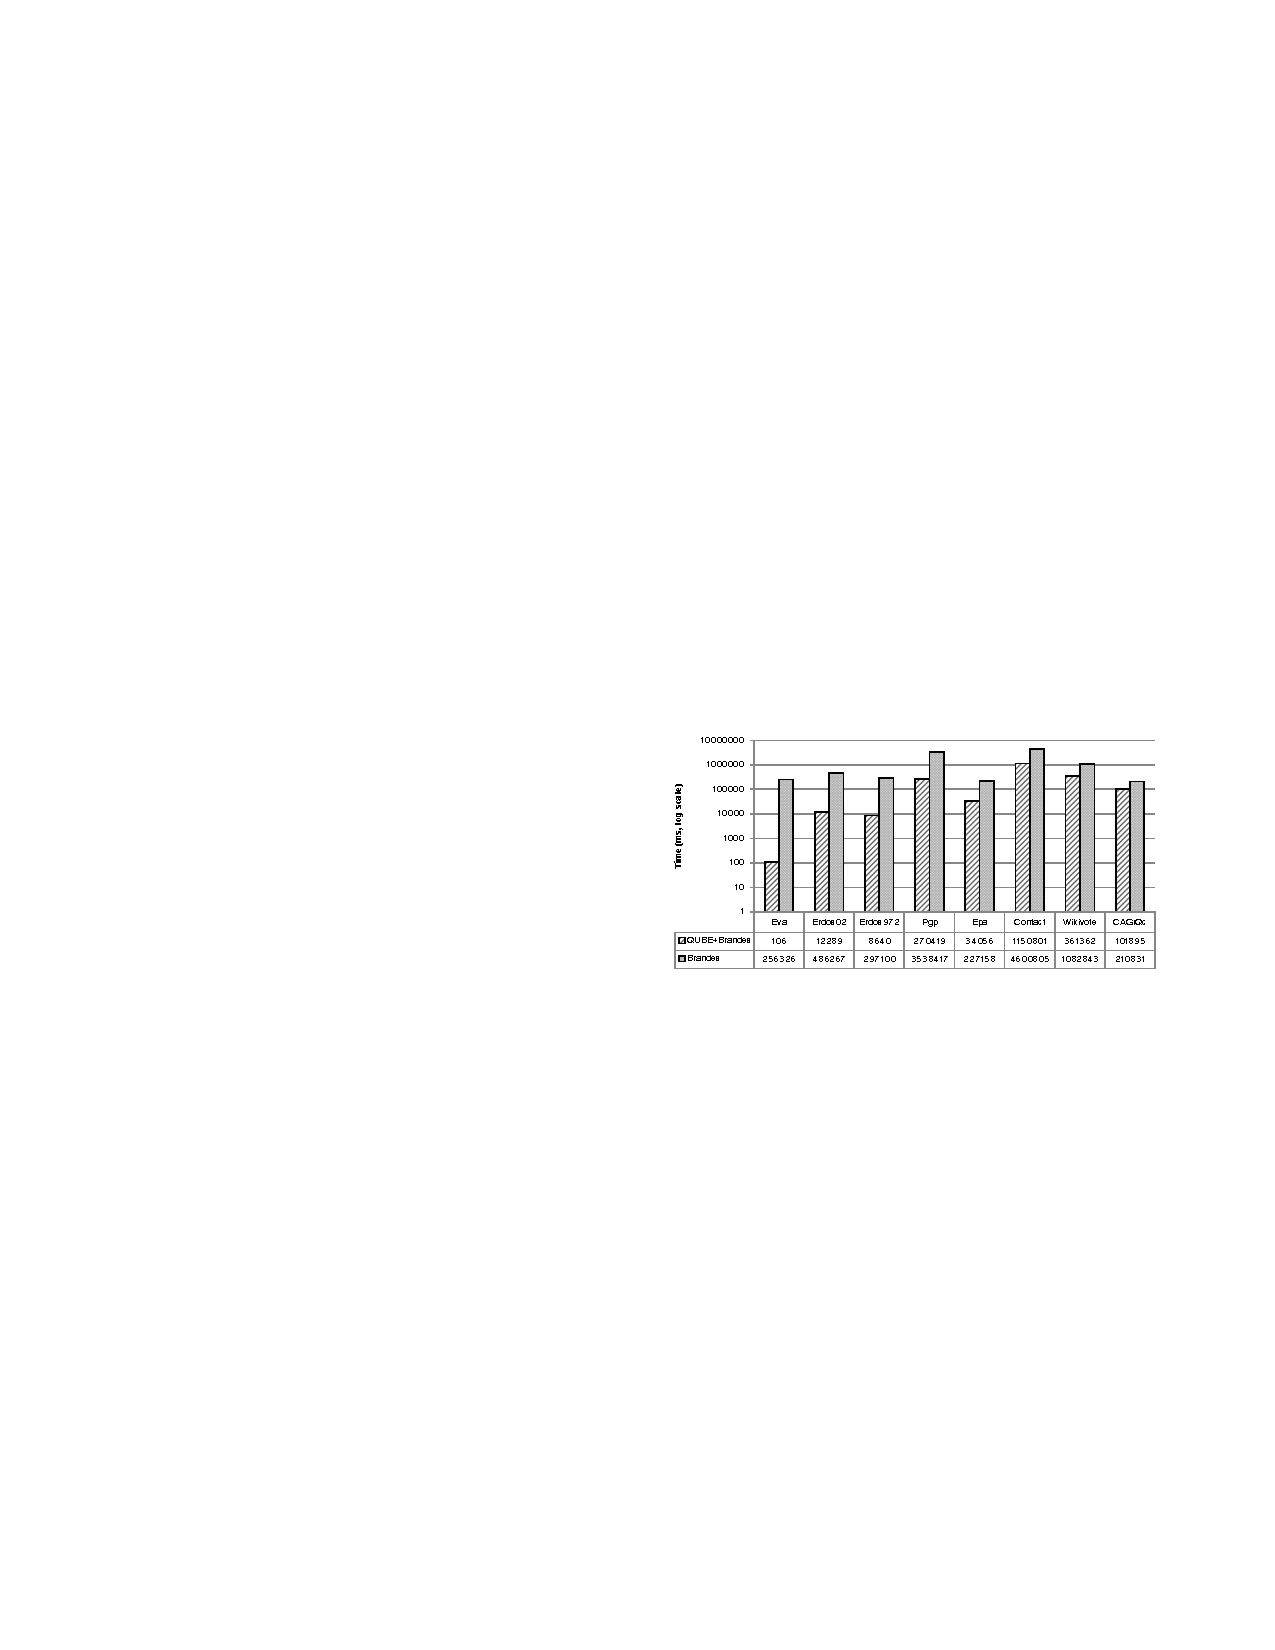
\includegraphics[width=\textwidth, height=0.6\textheight, keepaspectratio]{imgs/qube-results2}
  \end{figure}
  
  \begin{itemize}
    \item Improvement depends highly on structure of the graph (bi-connectedness)
    \item From 2 orders of magnitude (best) to 2 times (worst) faster than Brandes'
  \end{itemize}
    
\end{frame}


%% Kas et al.
\begin{frame}
  \frametitle{Incremental Algorithm for Updating Betweenness Centrality in Dynamically Growing Networks}
  \centering
  \vfill
  {\huge M. Kas, M. Wachs, K. M. Carley, L. R. Carley}
  \vfill
  {\large ASONAM '13: International Conference on Advances \\in Social Networks analysis and Mining}
\end{frame}


\begin{frame}
  \frametitle{Intuition}
  
  \begin{itemize}
    \item Extend an existing dynamic all-pairs shortest path algorithm to betweenness
    \item G. Ramalingam and T. Reps, ``\emph{On the Computational Complexity of Incremental Algorithms},'' CS, Univ. of Wisconsin at Madison, Tech. Report 1991
    \item Relevant quantities: number of shortest paths \paths, distances \dist, predecessors \pred
    \item Keep a copy of the old quantities while updating
  \end{itemize}
    
\end{frame}


\begin{frame}
  \frametitle{Edge update}
  
  \begin{itemize}
    \item Compute new shortest paths from updated endpoints $(v,w)$
    \item If a new shortest path of the same length is found, updated number of paths as
  \end{itemize}
  {\Large
  \begin{align*}
    \paths_{st} = \paths_{st} + \paths_{sv} \times \paths_{wt}
  \end{align*}
  }
    \begin{itemize}
    \item If a new \emph{shorter} shortest path to any node is found, update \dist, clear \paths
    \item Betweenness decreased if new shortest path found
    \item Edge betweenness updates backtrack via DFS over $\pred_s(t)$
  \end{itemize}
    {\Large
  \begin{align*}
    \betw(u) = \betw(u) - \paths_{su} \times \paths_{ut} / \paths_{st}
  \end{align*}
  }
\end{frame}


\begin{frame}
  \frametitle{Edge update}
  
  \begin{itemize}
    \item Complex bookkeeping: need to consider all affected vertices which have new alternative shortest paths of equal length (not covered in the original algorithm)
    \item Amend \pred during update propagation $\rightarrow$ concurrent changes to the \spath\dag
    \item Need to track now-unreachable nodes separately
  \end{itemize}
  
  \begin{itemize}
    \item After having fixed \dist, \paths, \betw, increase \betw due to new paths
    \item Update needed $\forall s,t \in V$ affected by changes (tracked from previous phase)
    \item Betweenness increase analogous to above decrease
  \end{itemize}
\end{frame}


\begin{frame}
  \frametitle{Results}

  \begin{figure}[t]
    \centering
    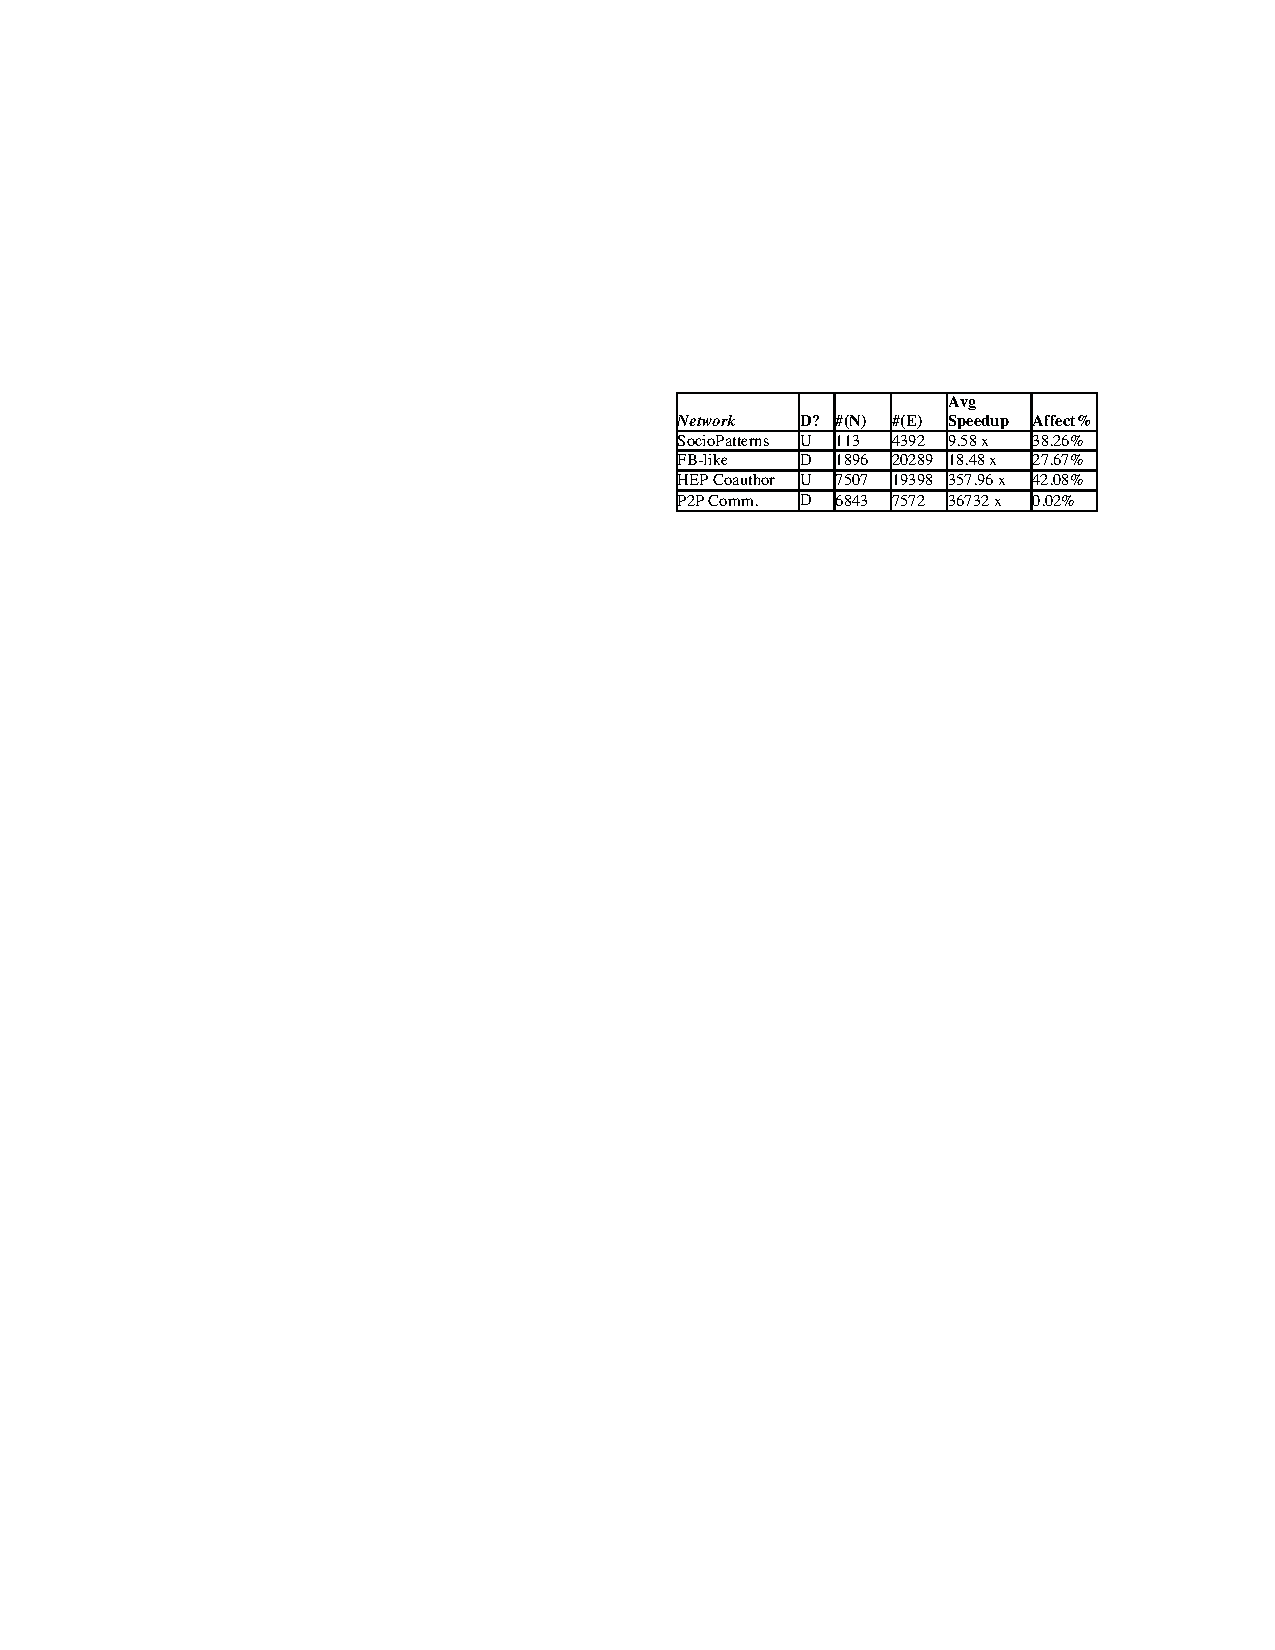
\includegraphics[width=\textwidth, height=0.7\textheight, keepaspectratio]{imgs/kas-results1}
    \caption{Speedup over Brandes' on real-world graphs}
  \end{figure}

  \begin{itemize}
    \item Speedup depends on topological characteristics (e.g., diameter, clust. coeff.)
  \end{itemize}
    
\end{frame}


\begin{frame}
  \frametitle{Comparison with QUBE}

  \begin{figure}[t]
    \centering
    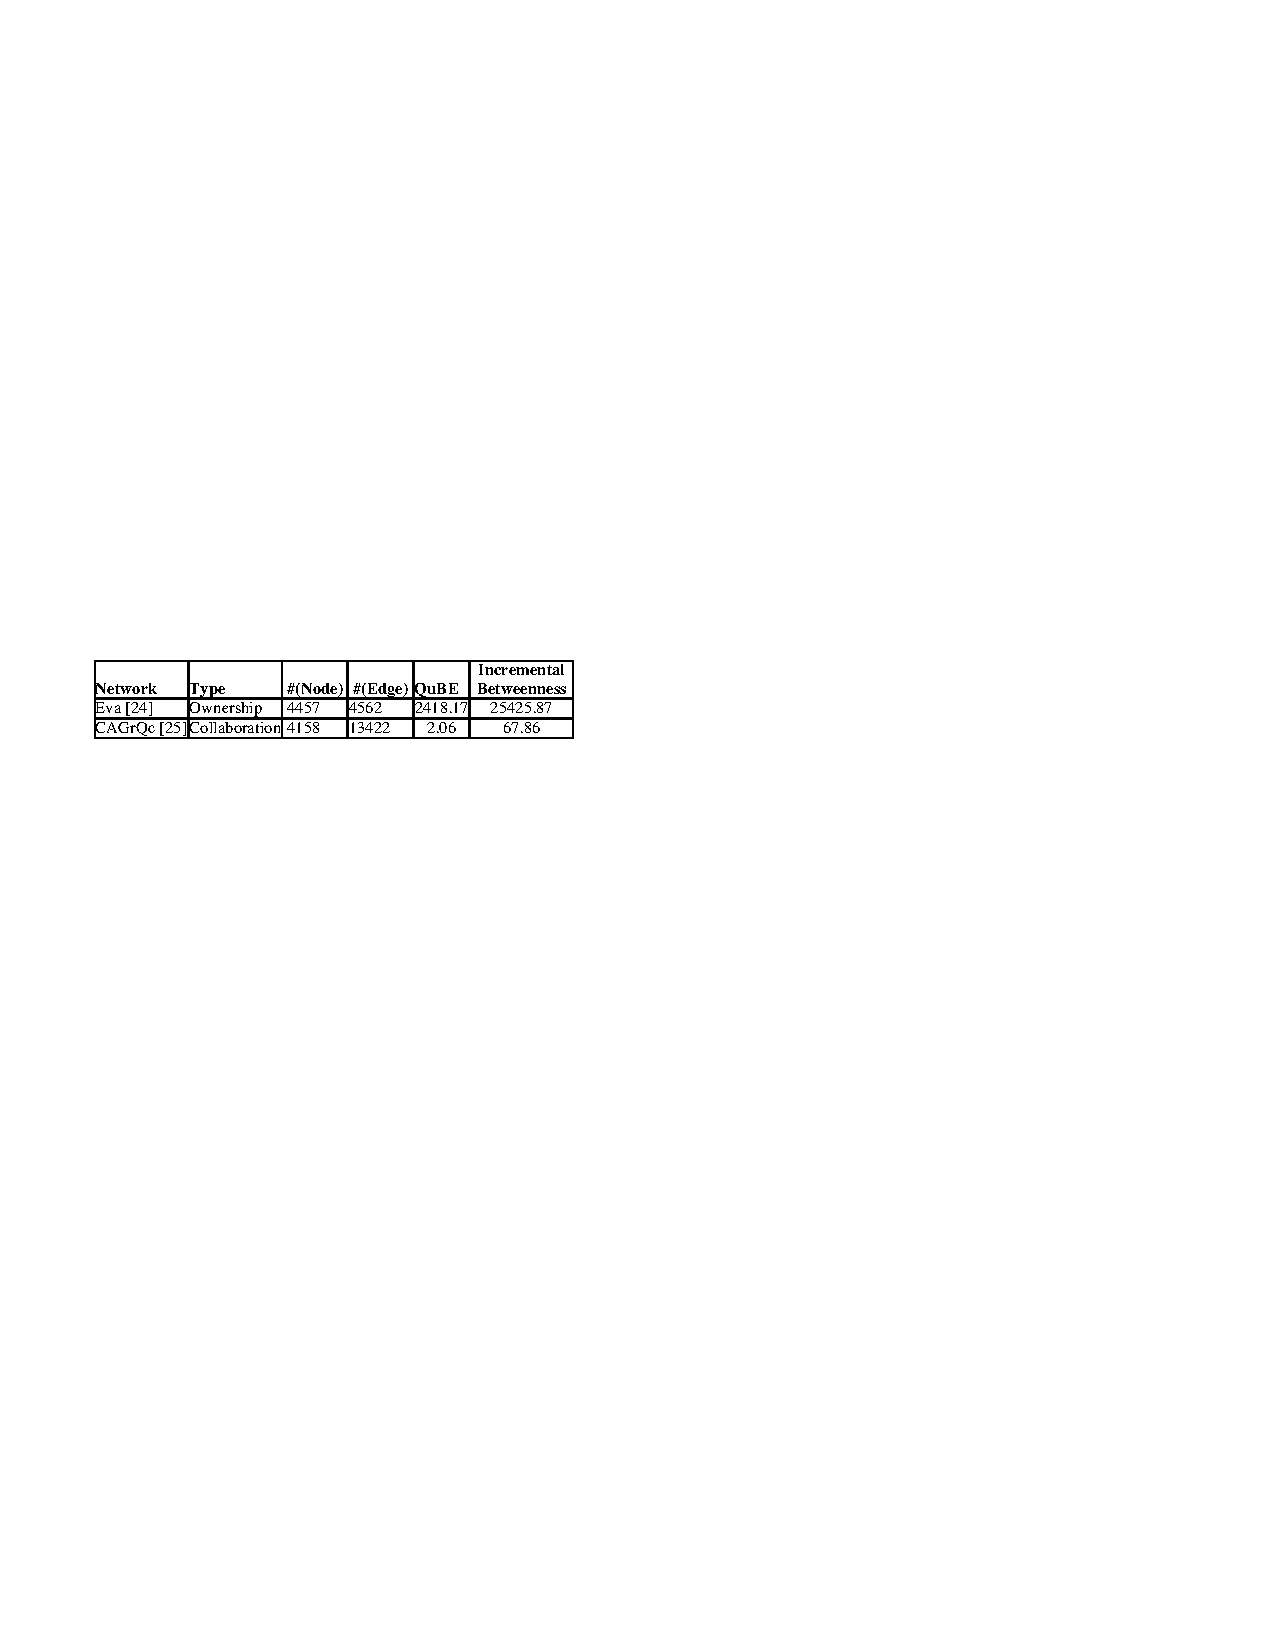
\includegraphics[width=\textwidth, height=0.7\textheight, keepaspectratio]{imgs/kas-results2}
%    \caption{}
  \end{figure}

  \begin{itemize}
    \item Datasets from the QUBE paper
    \item About 1 order of magnitude faster than QUBE
  \end{itemize}
    
\end{frame}


%% Green et al.
\begin{frame}
  \frametitle{A Fast Algorithm for Streaming Betweenness Centrality}
  \centering
  \vfill
  {\huge O. Green, R. McColl, D. A. Bader}
  \vfill
  {\large SocialCom '12: International Conference on Social Computing}
\end{frame}

\begin{frame}
  \frametitle{Intuition}

  \begin{itemize}
    \item Make Brandes' algorithm incremental
    \item Support only edge addition (on unweighted graphs)
    \item Keep additional data structures to avoid recomputing partial results
    \begin{itemize}
      \item Rooted \spdag for each source $s \in V$
      \item Depth in the tree for $t$ = distance of $t$ from $s$
    \end{itemize}
    \item Re-run parts of modified Brandes' algorithm on edge update
  \end{itemize}
    
\end{frame}


\begin{frame}
  \frametitle{Data structures}

  \begin{itemize}
    \item One \spdag (aka BFS dag) for each source $s \in V$, which contains for each other vertex $v \in V$:
    \begin{itemize}
      \item Distance \dist, paths \paths, dependencies \dep, predecessors \pred
      \item Additional per-level queues for exploration
    \end{itemize}
  \end{itemize}
  \begin{itemize}
    \item On addition of edge $u,v$ 3 cases:
    \begin{itemize}
      \item $|d_{su} - d_{sv}| = 0$ same~level
      \item $|d_{su} - d_{sv}| = 1$ adjacent~level
      \item $|d_{su} - d_{sv}| > 1$ non-adjacent~level
    \end{itemize}
  \end{itemize}
      
\end{frame}


\begin{frame}
  \frametitle{Same level addition}
  \begin{columns}[onlytextwidth]
  
    \begin{column}{0.5\textwidth}
      \begin{itemize}
        \item $|d_{su} - d_{sv}| = 0$
        \item Edge creates no new shortest paths
        \item No change to betweenness \\ due to this source
      \end{itemize}
    \end{column}
    
    \begin{column}{0.5\textwidth}
      \begin{figure}[t]
        \centering
        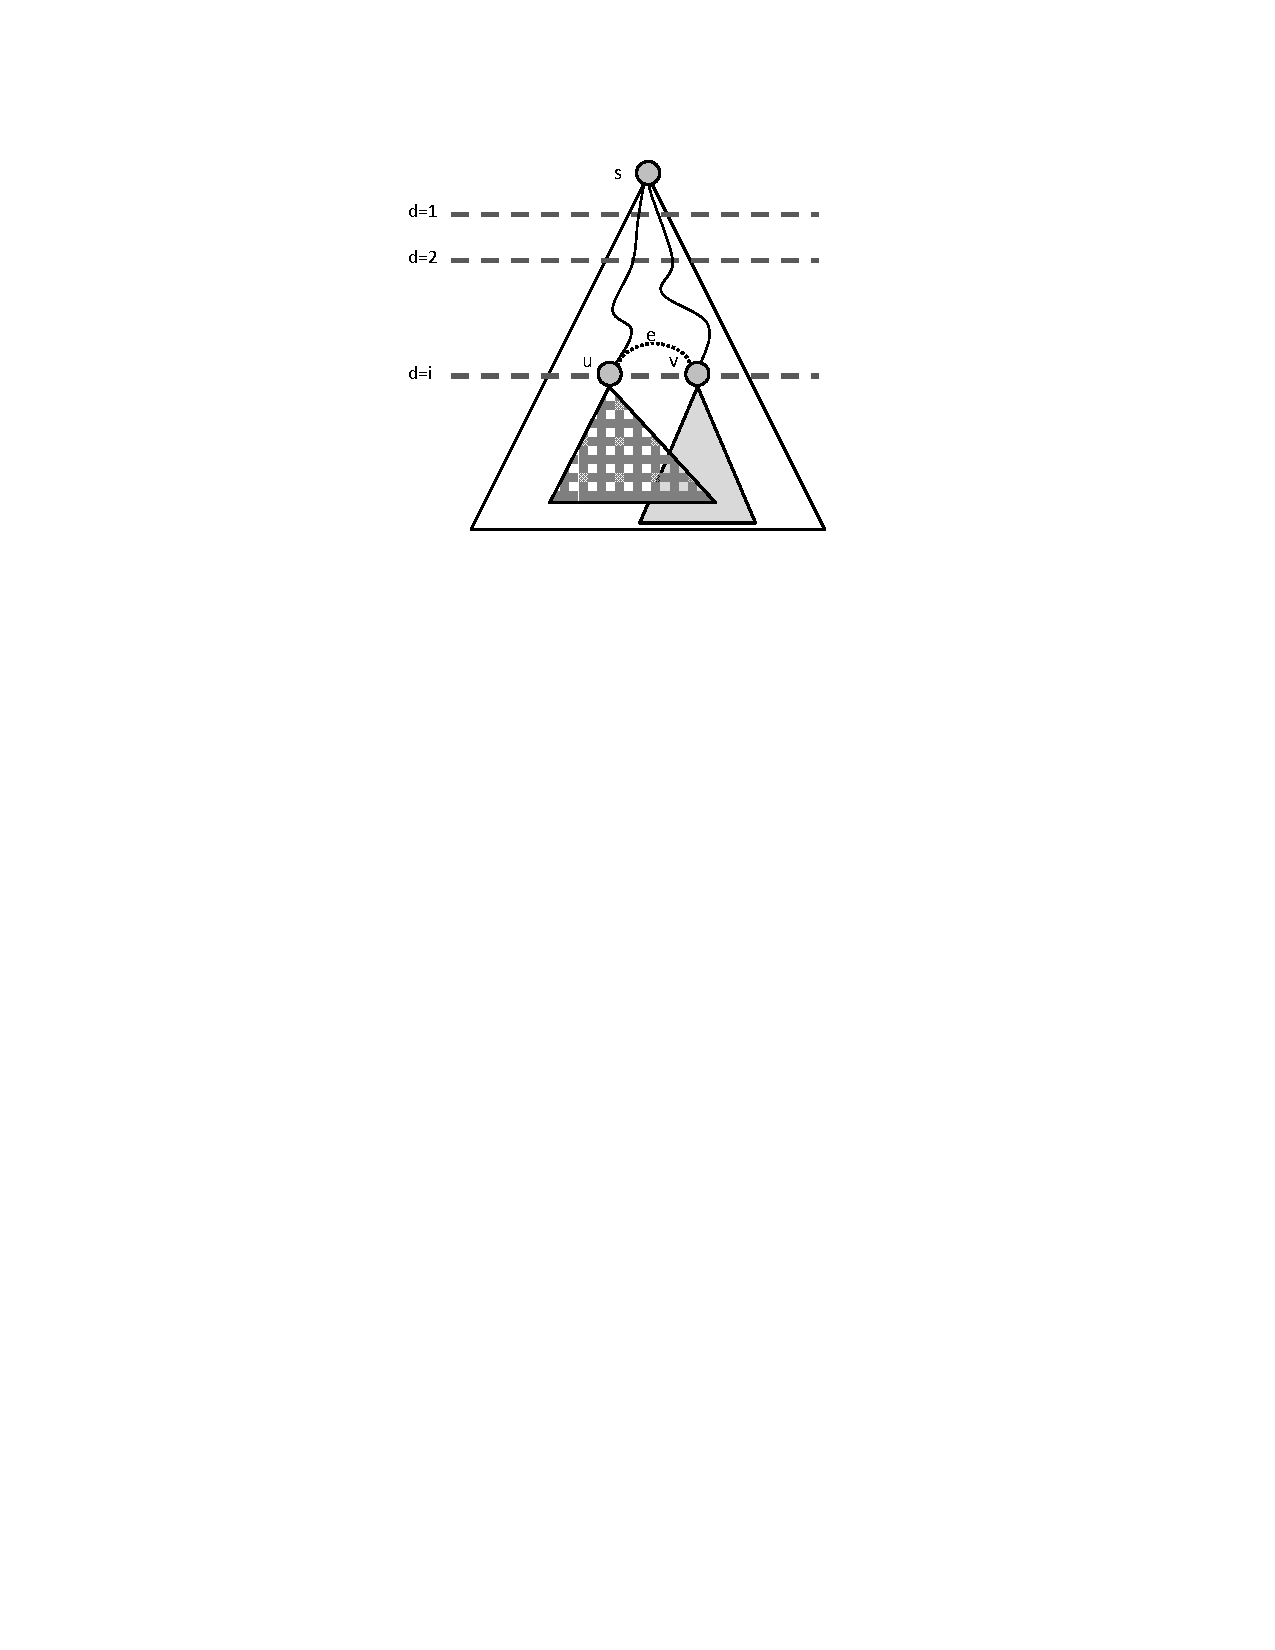
\includegraphics[width=\textwidth, height=\textheight, keepaspectratio]{imgs/green-0lvl-compressed}
      \end{figure}
    \end{column}
  \end{columns}
  
\end{frame}


\begin{frame}
  \frametitle{Adjacent level addition}
  \begin{columns}[onlytextwidth]
  
    \begin{column}{0.5\textwidth}
      \begin{itemize}
        \item $|d_{su} - d_{sv}| = 1$
        \item Let $u_{high} = u ,\, u_{low} = v$
        \item Edge creates new shortest paths
        \item \spdag unchanged
        \item Changes in \paths confined to sub-dag rooted in $u_{low}$
        \item Changes in \dep also spread above to decrease old dependency and account for new dependency
        \item Example: $w$ and predecessors have now only $\sfrac{1}{2}$ of dependency on sub-dag rooted in $u_{low}$
      \end{itemize}
    \end{column}
    
    \begin{column}{0.5\textwidth}
      \begin{figure}[t]
        \centering
        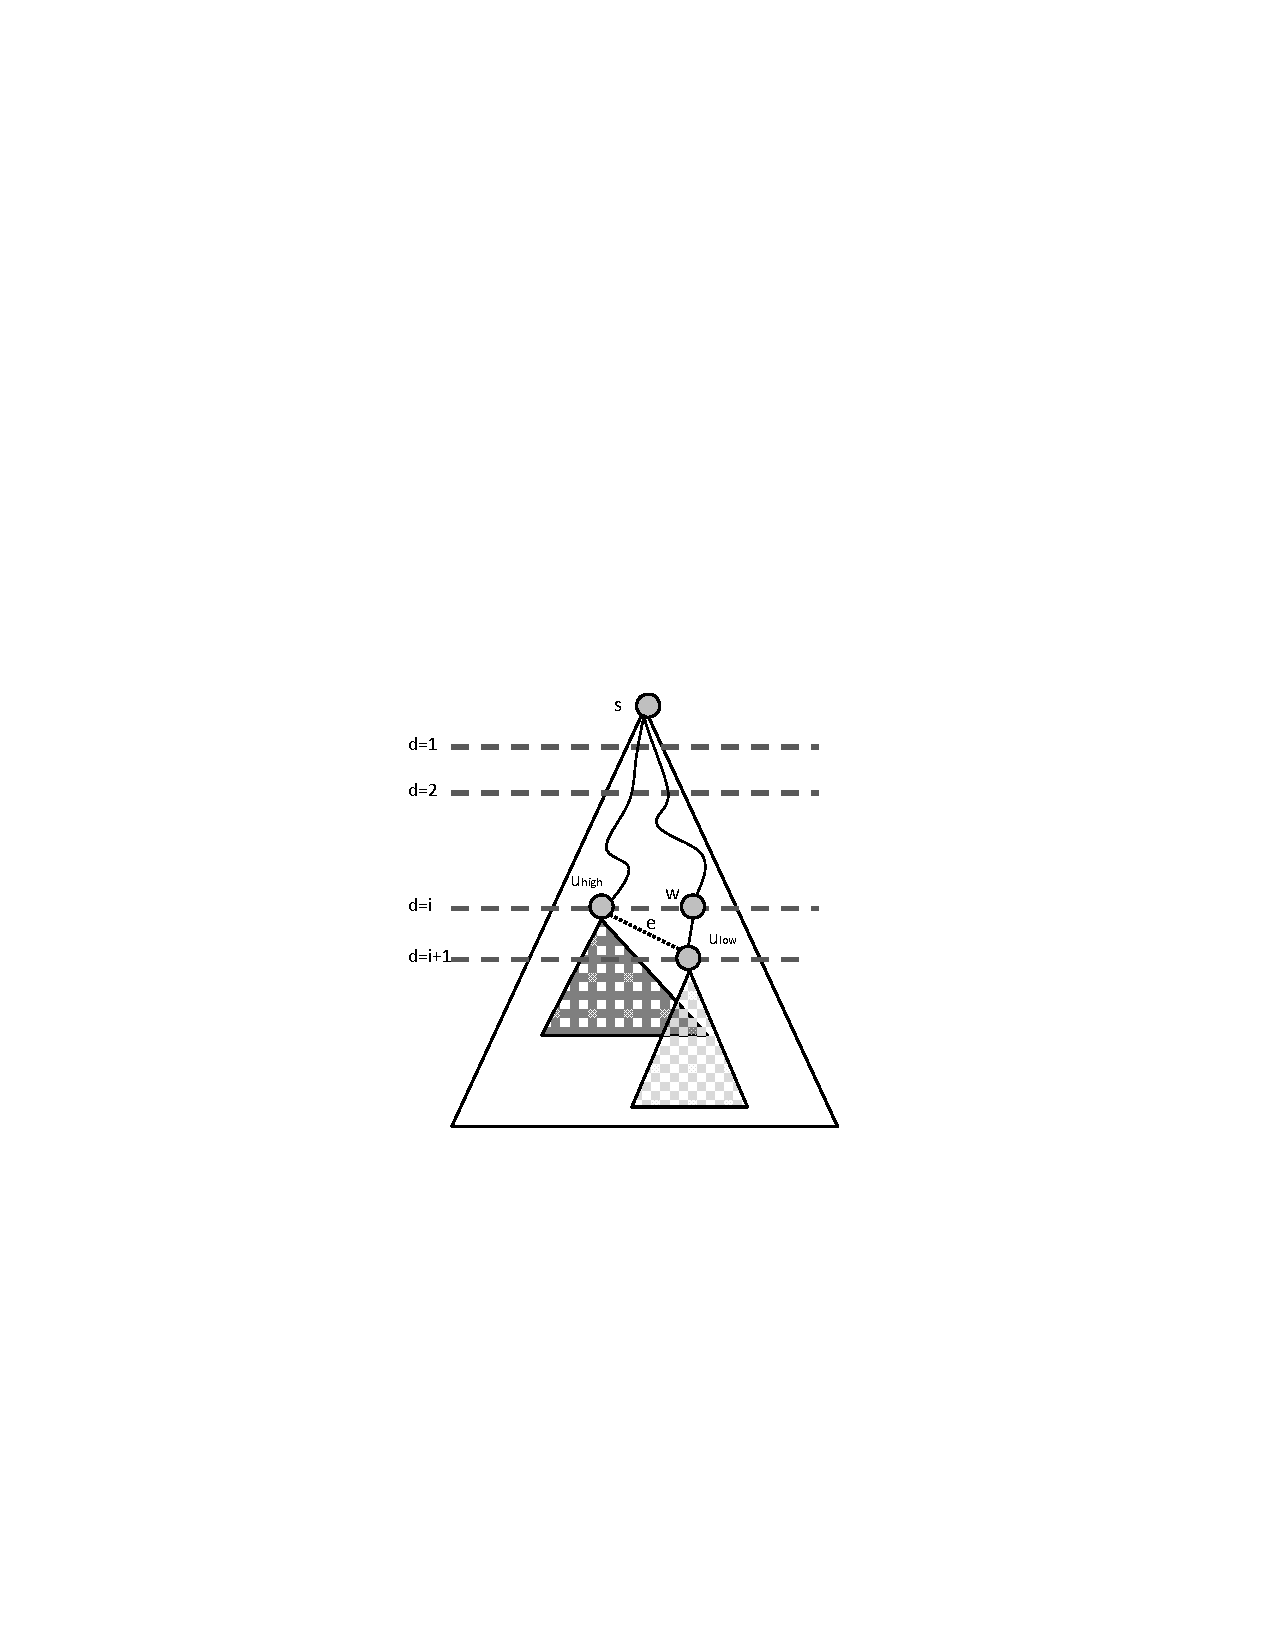
\includegraphics[width=\textwidth, height=\textheight, keepaspectratio]{imgs/green-1lvl-compressed}
      \end{figure}
    \end{column}
  \end{columns}
    
\end{frame}


\begin{frame}
  \frametitle{Algorithm}
  \begin{columns}[onlytextwidth]
  
    \begin{column}{0.3\textwidth}
      \begin{itemize}
        \item During exploration:
        \begin{itemize}
          \item Fix \paths
          \item Mark visited vertices
          \item Enqueue for further processing
        \end{itemize}
      \end{itemize}
      \begin{itemize}
        \item During backtracking:%
        \begin{itemize}
          \item Fix \dep and \betw
          \item Recurse up the whole \spdag
        \end{itemize}
      \end{itemize}
    \end{column}
    
    \begin{column}{0.7\textwidth}
      \begin{figure}[t]
        \centering
%        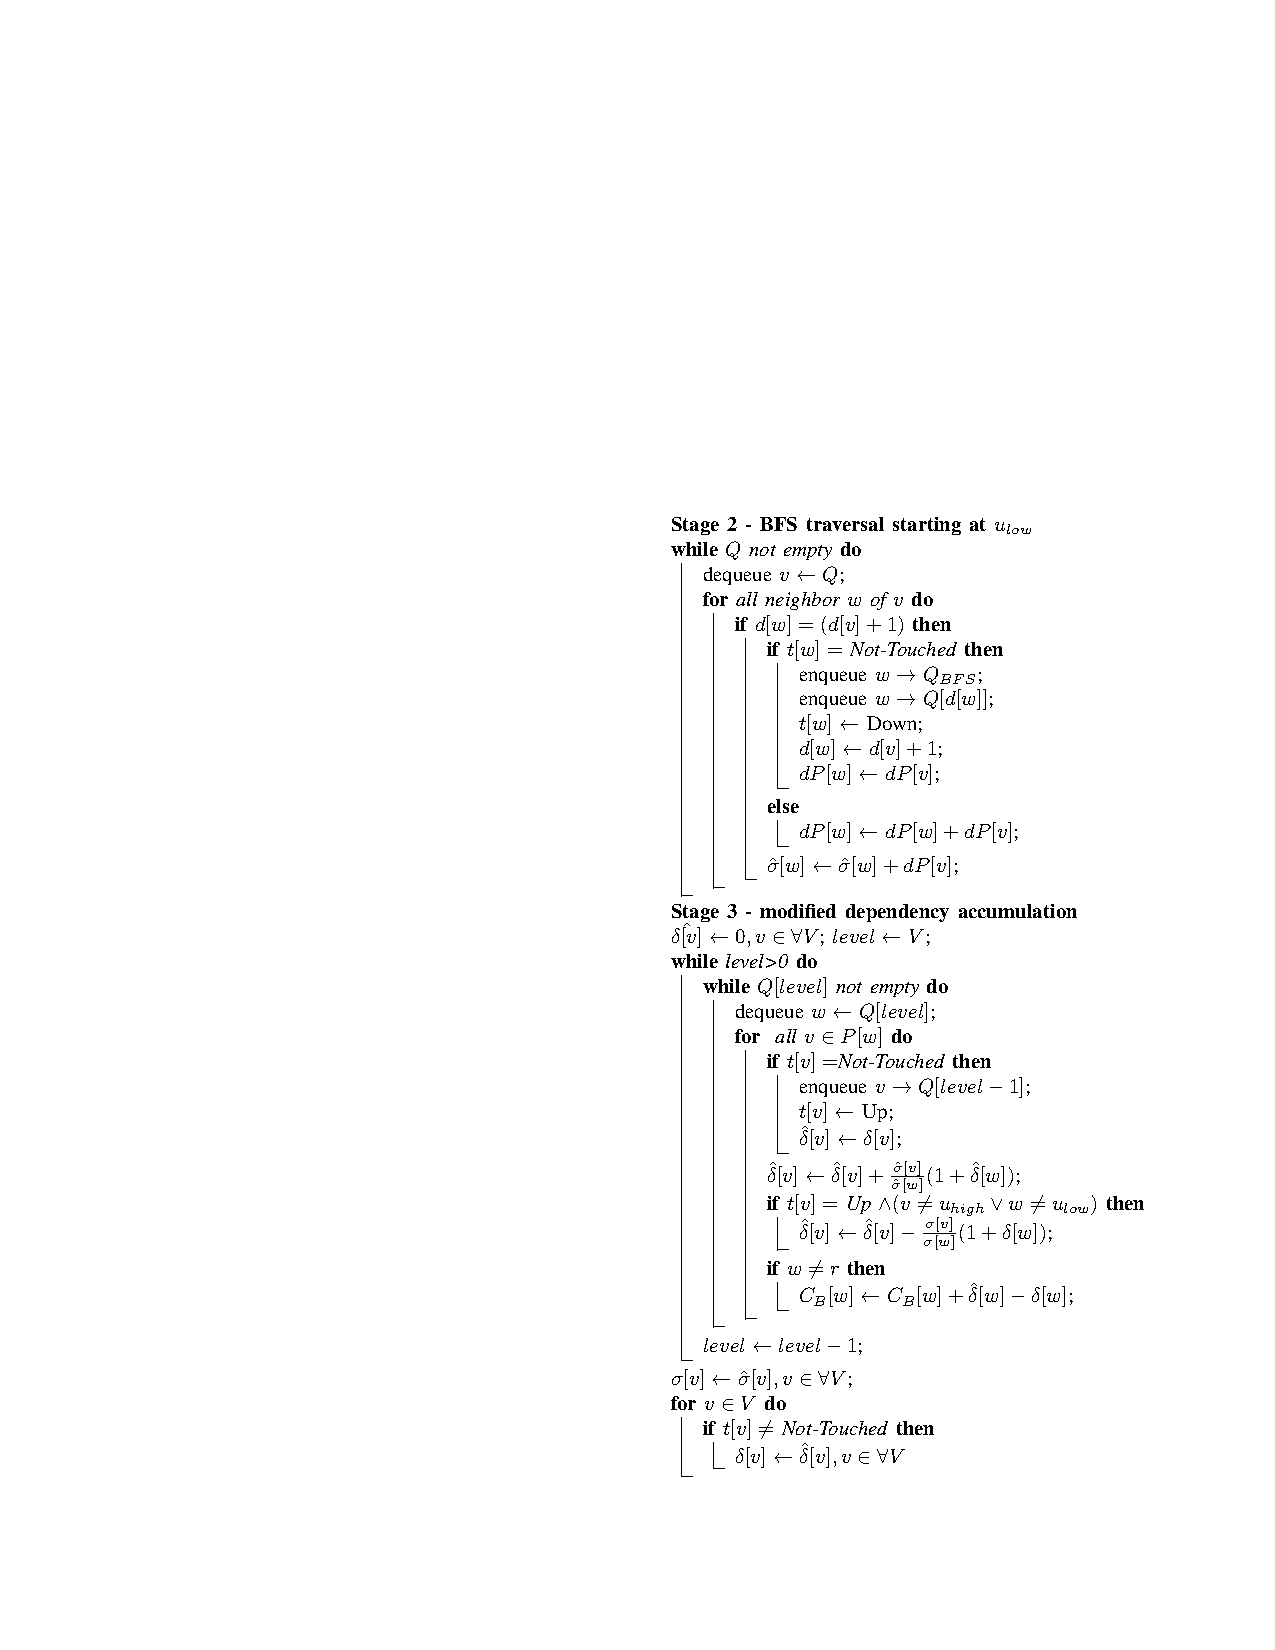
\includegraphics[width=\textwidth, height=0.8\textheight, keepaspectratio]{imgs/green-algo}
        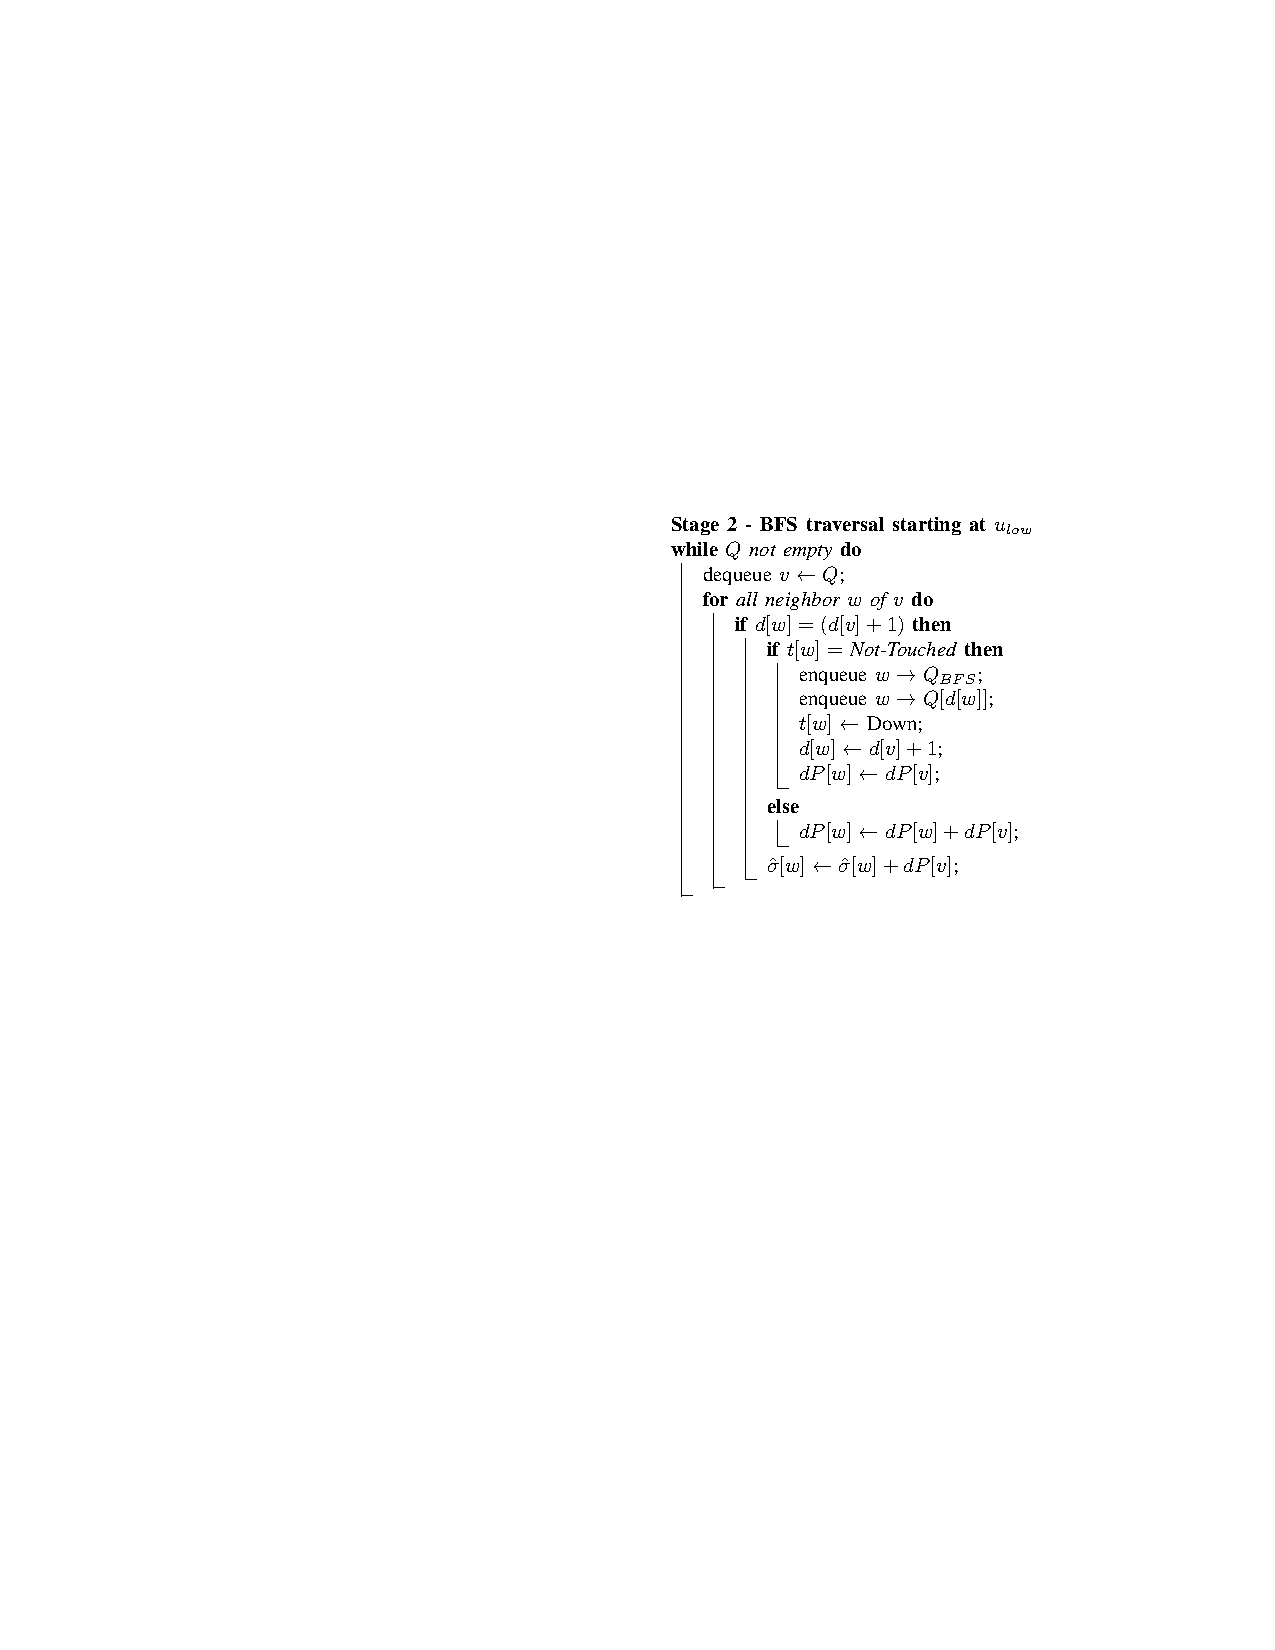
\includegraphics[width=0.45\textwidth, height=0.8\textheight, keepaspectratio, valign=t]{imgs/green-algo1}
        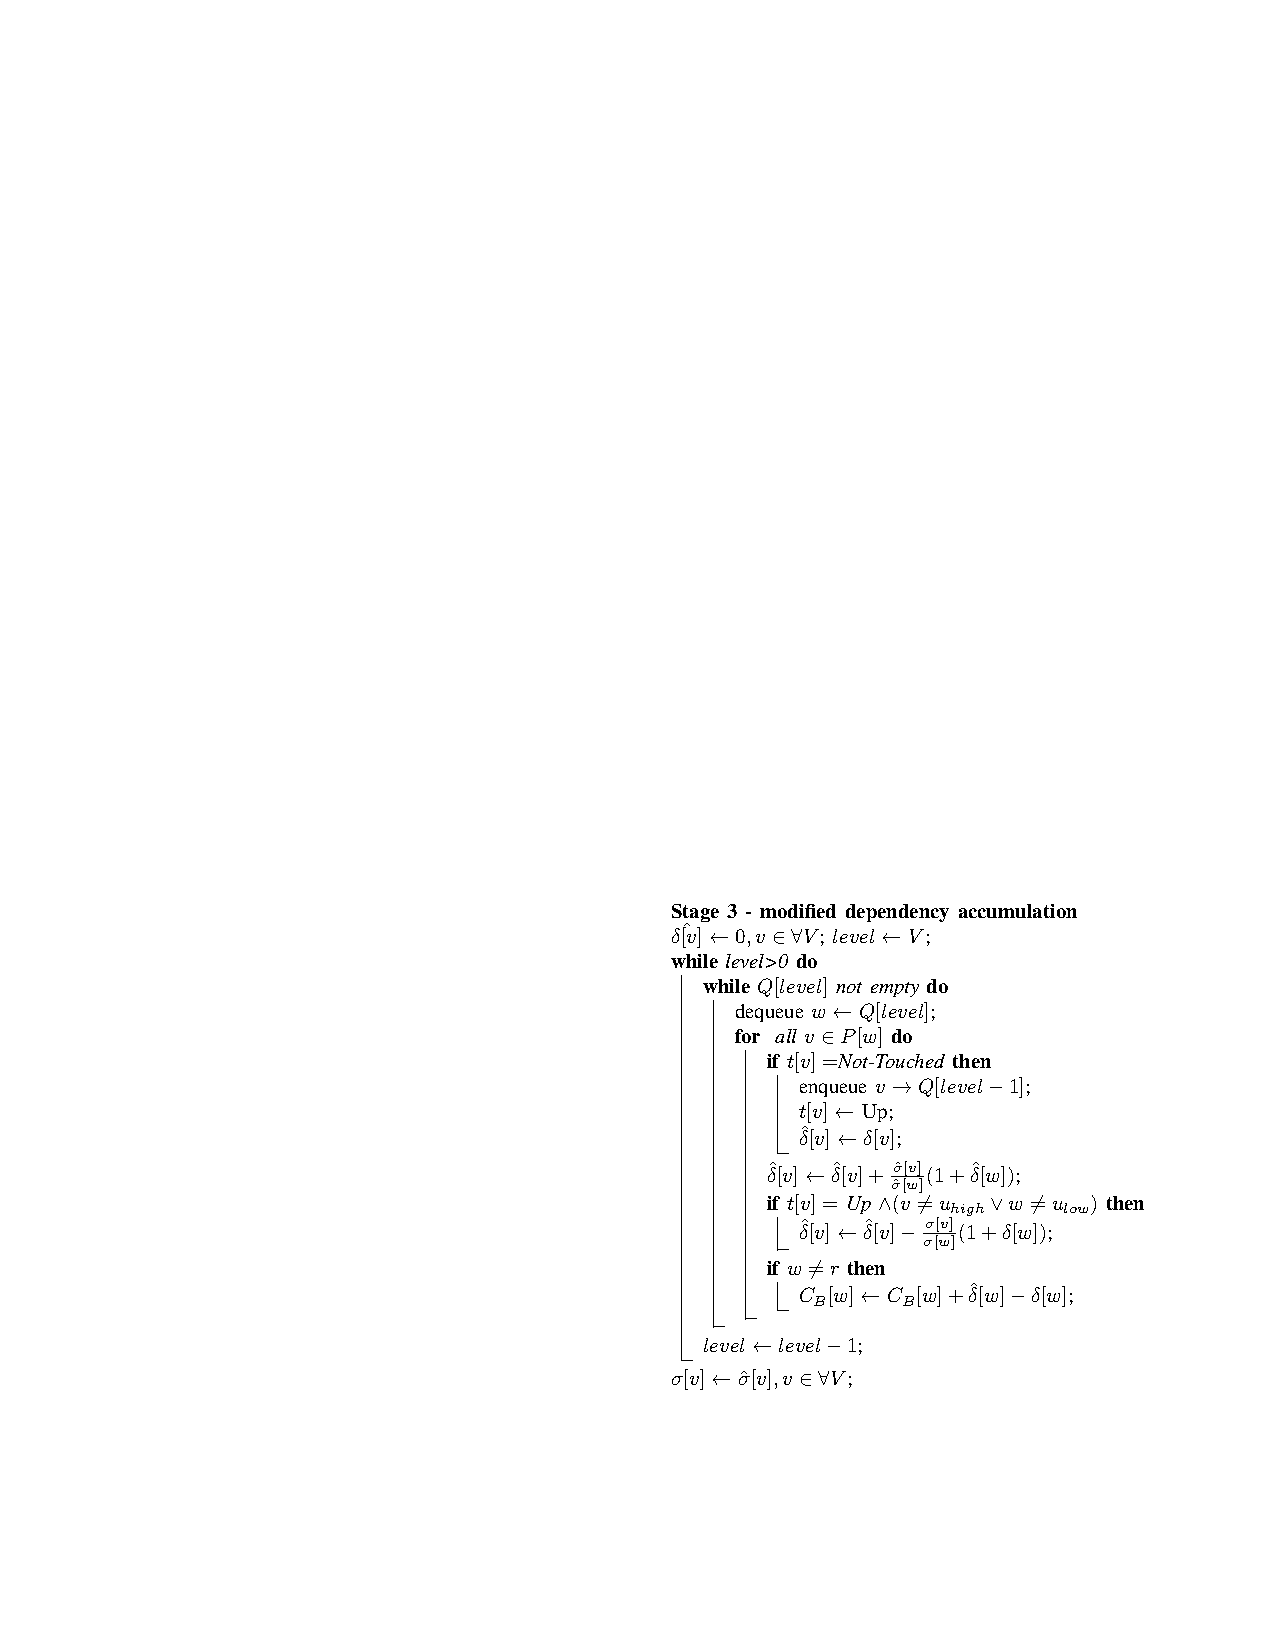
\includegraphics[width=0.6\textwidth, height=0.8\textheight, keepaspectratio, valign=t]{imgs/green-algo2}
      \end{figure}
    \end{column}
  \end{columns}
\end{frame}


\begin{frame}
  \frametitle{Non-adjacent level addition}
  
  \begin{columns}[onlytextwidth]
  
    \begin{column}{0.5\textwidth}
      \begin{itemize}
        \item $|d_{su} - d_{sv}| > 1$
        \item Edge creates new shortest paths
        \item Changes to \spdag (new distances)
        \item Algorithm only sketched \\ (most details missing)
      \end{itemize}
    \end{column}
    
    \begin{column}{0.5\textwidth}
      \begin{figure}[t]
        \centering
        \includegraphics<1>[width=\textwidth, height=0.8\textheight, keepaspectratio]{imgs/green-2lvl-before-compressed}
          \transdissolve<2>
          \transduration{2}
        \includegraphics<2>[width=\textwidth, height=0.8\textheight, keepaspectratio]{imgs/green-2lvl-after-compressed}
      \end{figure}
    \end{column}
  \end{columns}
    
\end{frame}


\begin{frame}
  \frametitle{Complexity}

  \begin{itemize}
    \item Time: $O(n^2 + nm)$ $\leftarrow$ same as Brandes'
    \item In practice, algorithm is much faster
  \end{itemize}
  \begin{itemize}
    \item Space: $O(n^2 + nm)$ $\leftarrow$ higher than Brandes'
    \item For each source, a \spdag of complexity $n + n$ 
  \end{itemize}
    
\end{frame}


\begin{frame}
  \frametitle{Results}
  
  \begin{figure}[t]
    \centering
    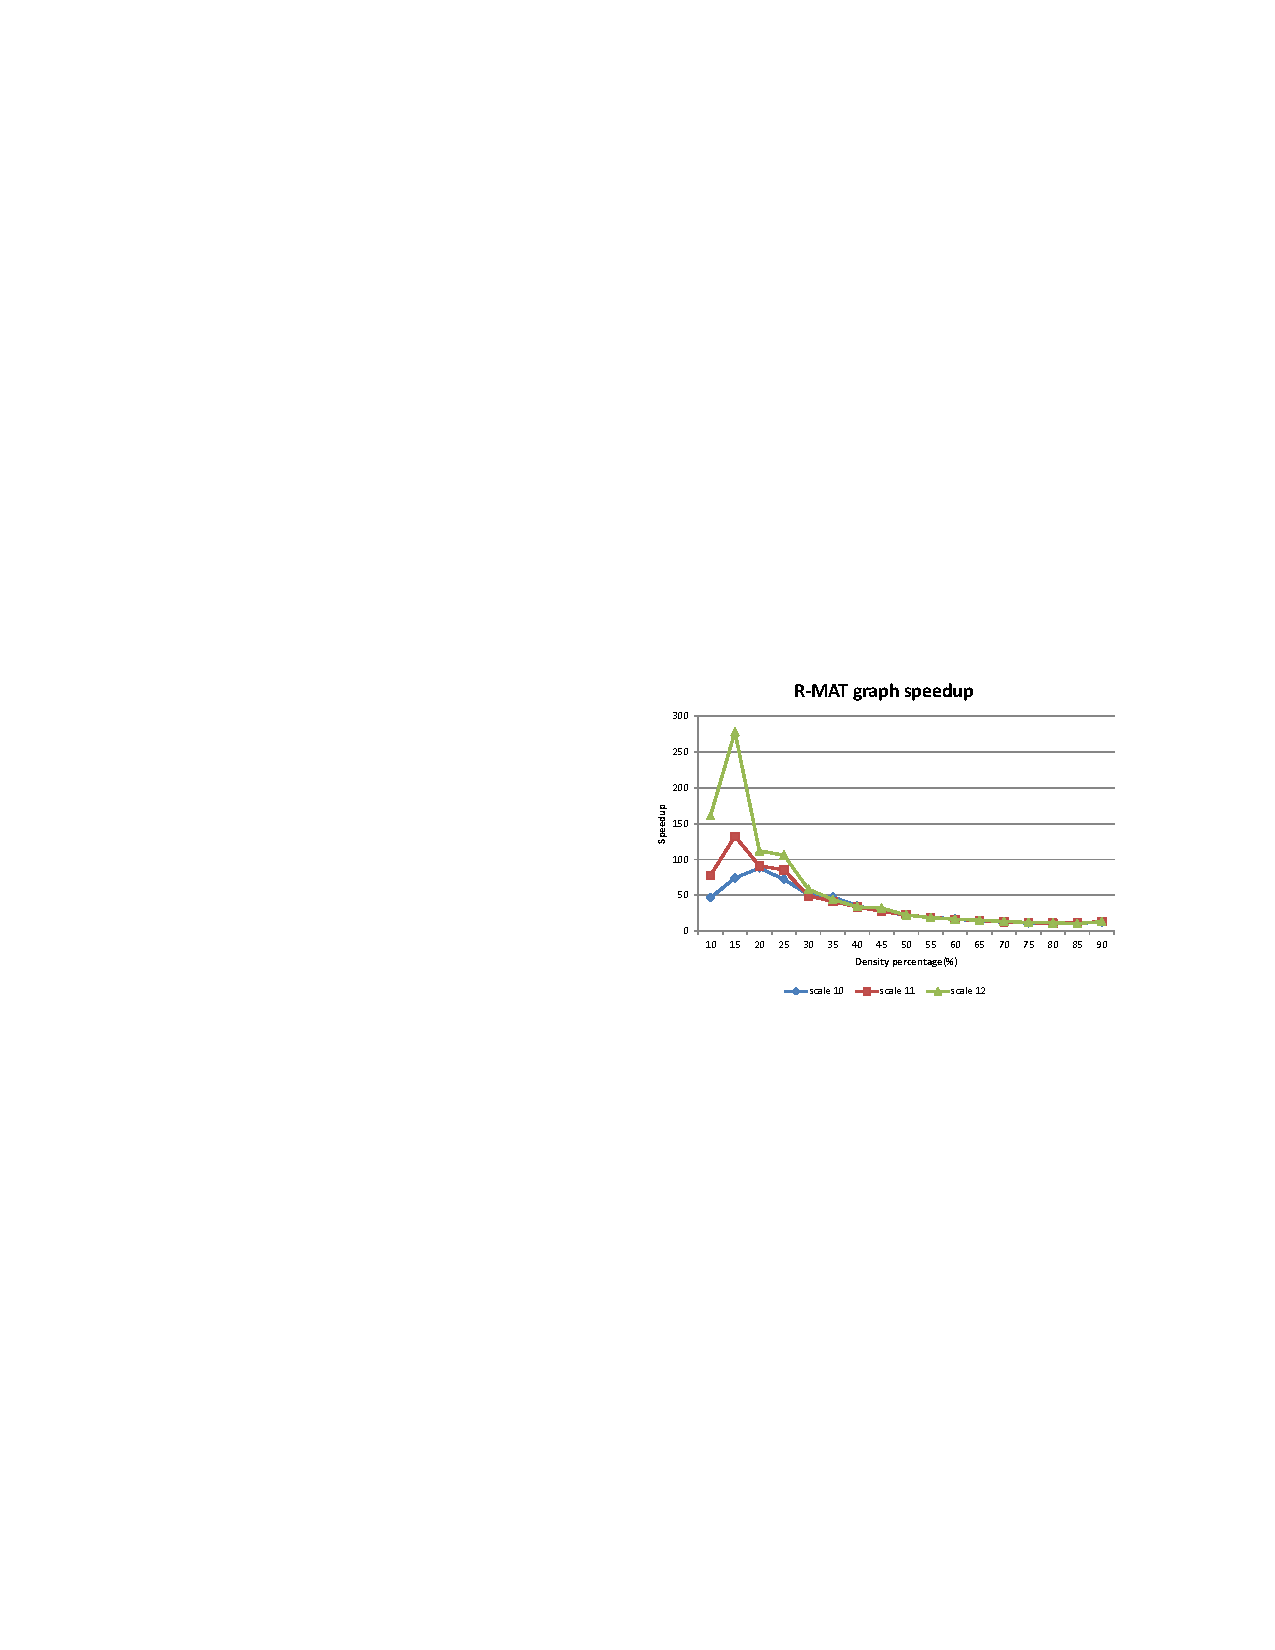
\includegraphics[width=\textwidth, height=0.7\textheight, keepaspectratio]{imgs/green-results1}
    \caption{Speedup over Brandes' on synthetic graphs ($n = 4096$)}
  \end{figure}
    
\end{frame}


\begin{frame}
  \frametitle{Conclusions}

  \begin{itemize}
    \item Up to 2 orders of magnitude speedup
    \item Quadratic space bottleneck
  \end{itemize}
    
\end{frame}
